\chapter{Agil.It}

No capítulo anterior foi detalhado as principais características da estrutura e organização do código fonte do sistema.
A seguir será apresentado as principais telas e funcionalidades disponíveis aos usuários.

\section{WEB}
A aplicação WEB tem seu foco na parte administrativa e gerencial do sistema, através dela o administrador poderá realizar os cadastros, assinaturas e acompanhar as situações de todas as ordens que estão em andamento.
\subsection{Cadastros do sistema}

\begin{figure}[H]
	\caption{\label{web-cadastros}Cadastros do Sistema}
	\begin{center}
		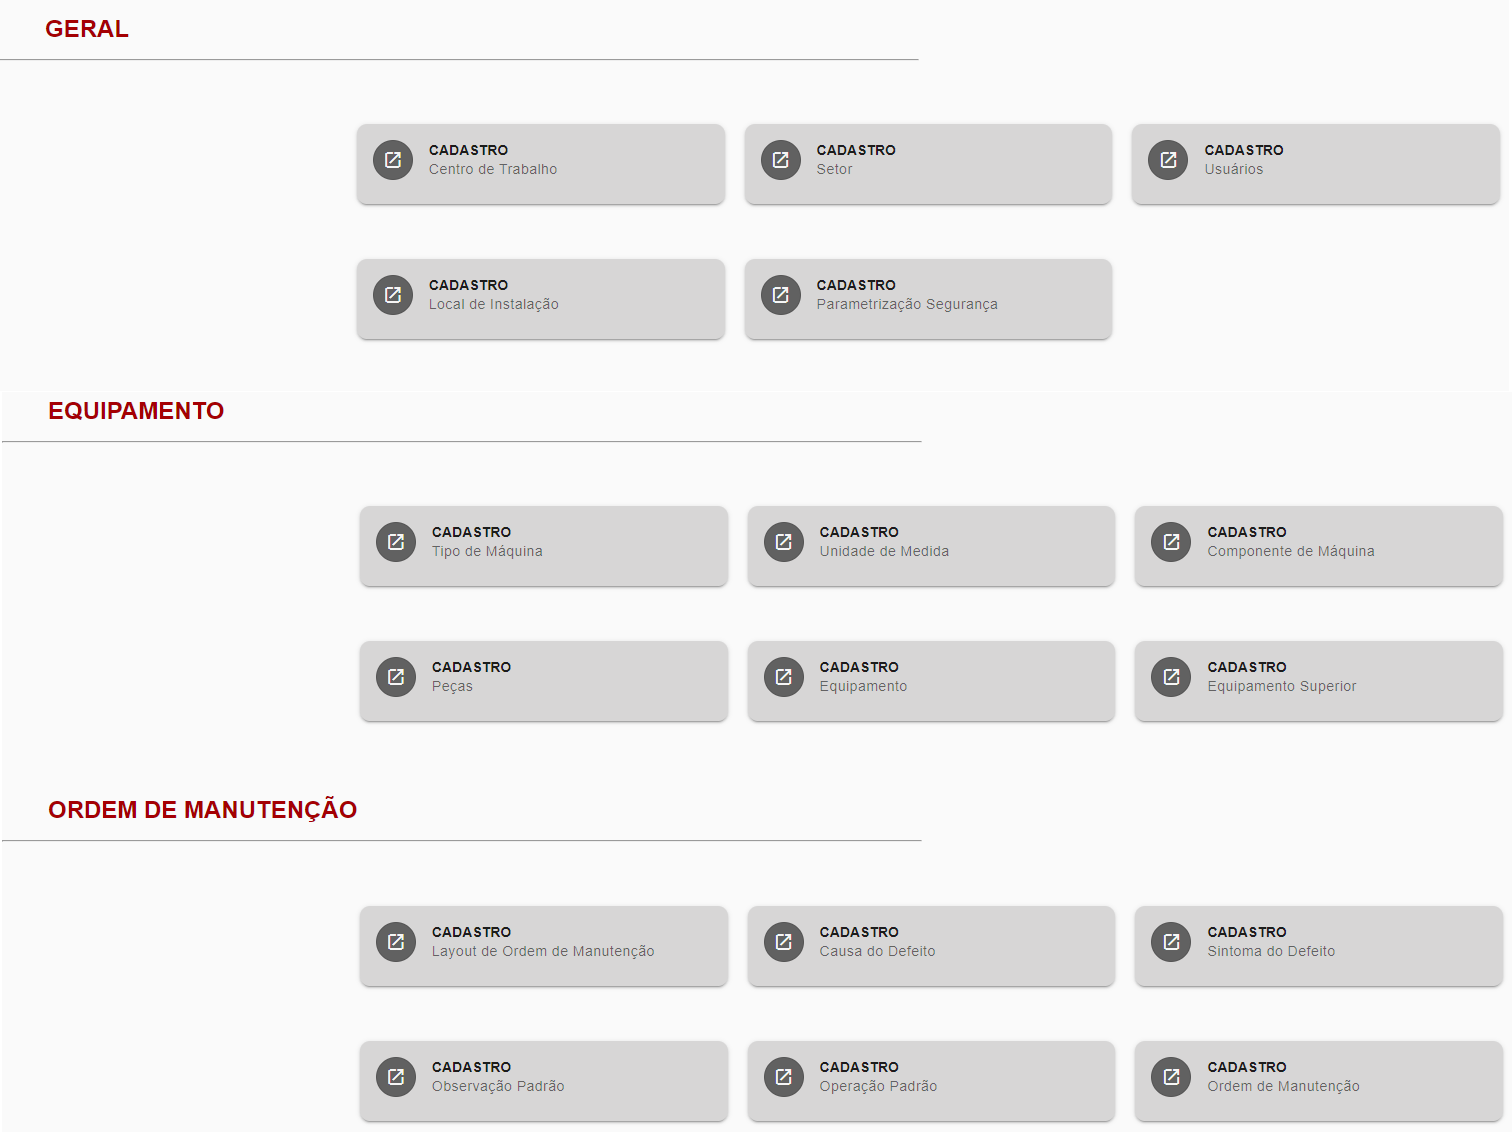
\includegraphics[scale=0.40]{./Figuras/agil.it/web-cadastros.png}
	\end{center}
	\legend{Fonte: os autores (2020)}
\end{figure}

A figura \ref{web-cadastros} mostra a lista de cadastros disponíveis no sistema.

\begin{figure}[H]
	\caption{\label{web-cadastro-equipamento}Cadastro de Equipamento}
	\begin{center}
		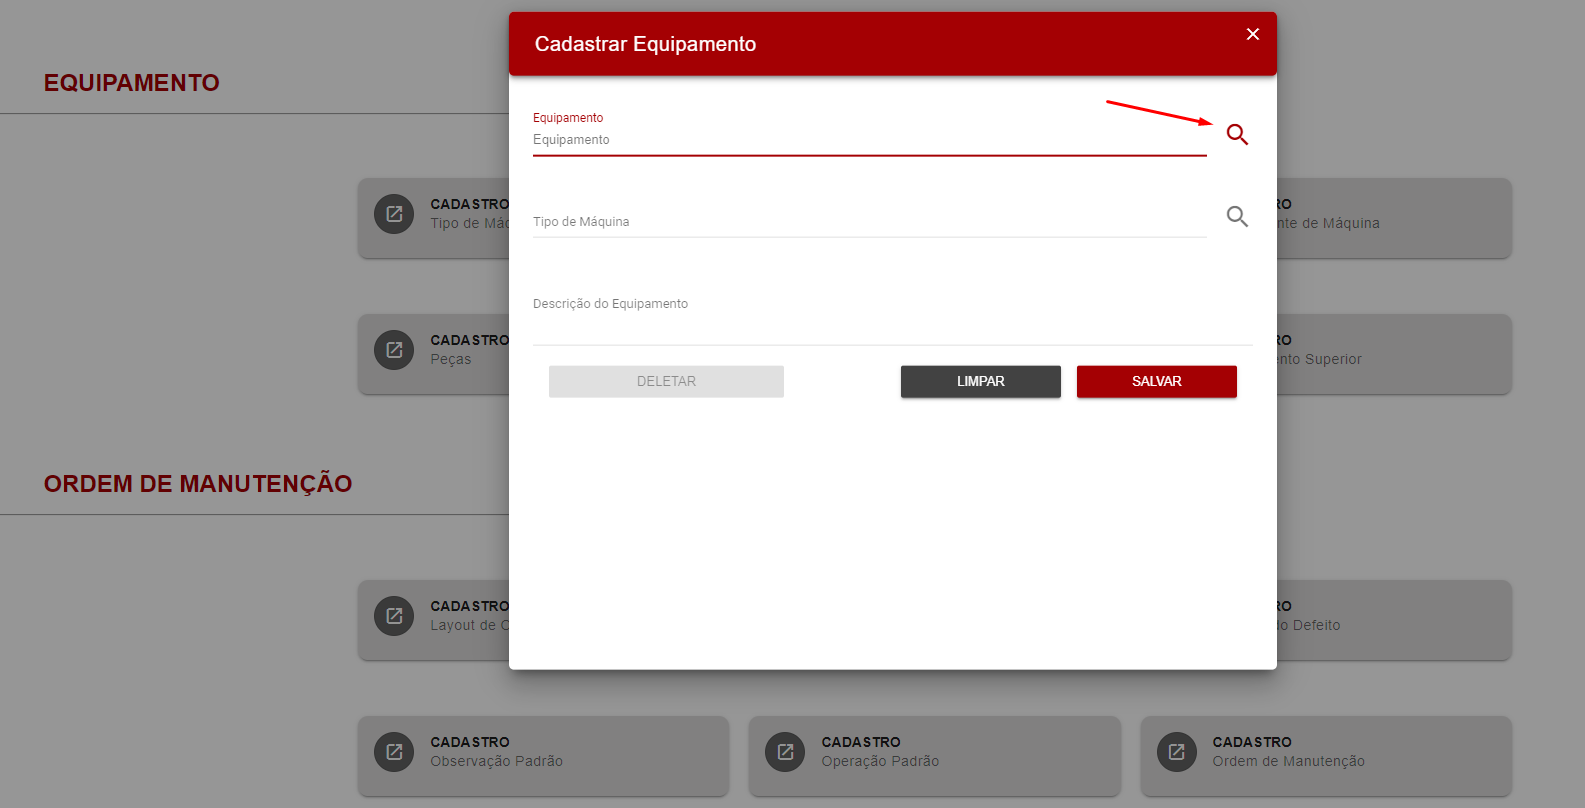
\includegraphics[scale=0.40]{./Figuras/agil.it/web-cadastro-equipamento.png}
	\end{center}
	\legend{Fonte: os autores (2020)}
\end{figure}

A figura \ref{web-cadastro-equipamento} mostra o cadastro de Equipamento, as demais telas de cadastro do sistema seguem o mesmo padrão, nas cores vermelho e branco e com campos de auto preenchimento conforme as informações são digitadas, os usuários conseguem efetuar a busca de dados de uma forma fácil e ágil. Os cadastros possuem também uma tela de consulta que fica visível ao clicar no ícone de lupa disponível no lado direito dos campos de auto preenchimento.
Entretanto, a tela Cadastro de Ordem de Manutenção é a única que contém abas para facilitar no preenchimento das informações por ser um cadastro mais extenso e trabalhoso.

Na figura \ref{web-search-table} mostra um exemplo de como fica a visualização da tela de consulta no cadastro de Equipamentos.

\begin{figure}[H]
	\caption{\label{web-search-table}Consulta de Equipamento}
	\begin{center}
		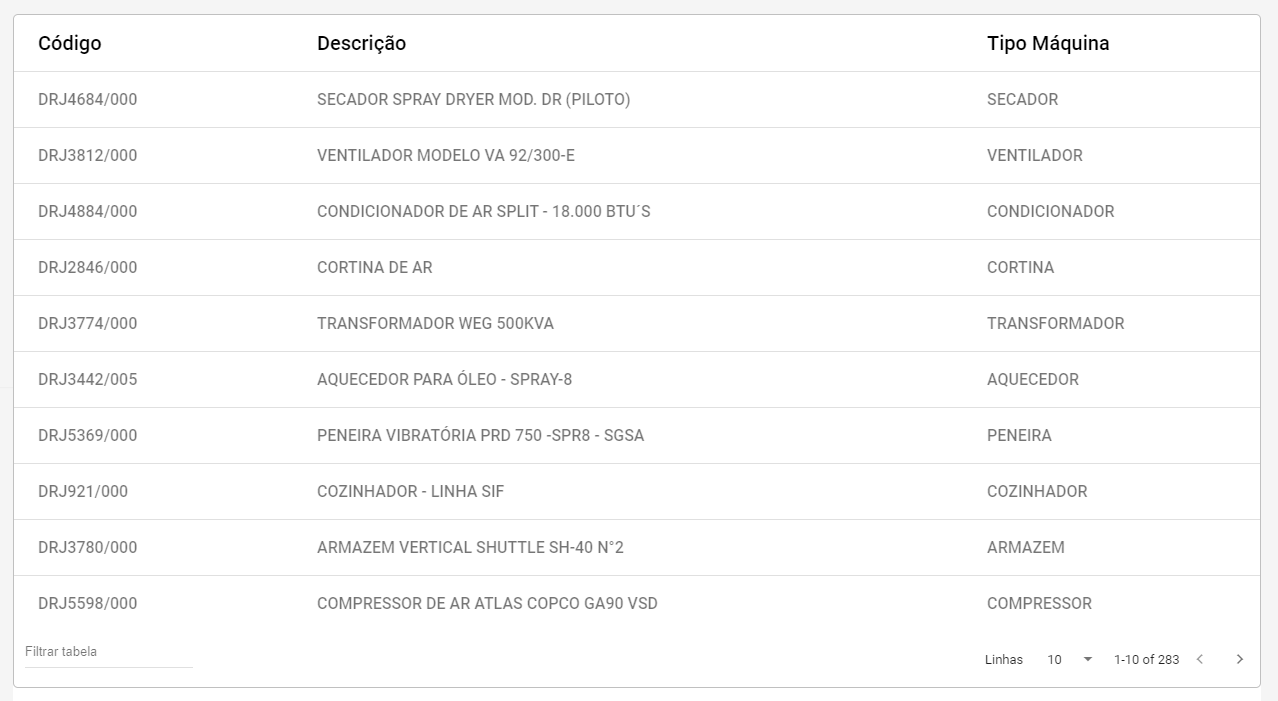
\includegraphics[scale=0.50]{./Figuras/agil.it/web-search-table.png}
	\end{center}
	\legend{Fonte: os autores (2020)}
\end{figure}

\subsection{Dashboard}

Essa tela tem como objetivo facilitar o monitoramento das ordens de manutenção, com a disponibilidade de filtros por data, status e prioridade os usuários conseguem encontrar o que desejam de uma forma muito mais rápida. Além disso, a Dashboard conta com duas opções de visualização das ordens listadas em tela, a primeira opção seria em forma de tabela com um filtro adicional por texto, conforme figura \ref{web-monitor-lista} e a segunda em forma de cards que contém cores para identificar a prioridade das ordens, conforme figura \ref{web-monitor-cards}.

\begin{figure}[H]
	\caption{\label{web-monitor-lista}Dashboard: Visualização por tabela}
	\begin{center}
		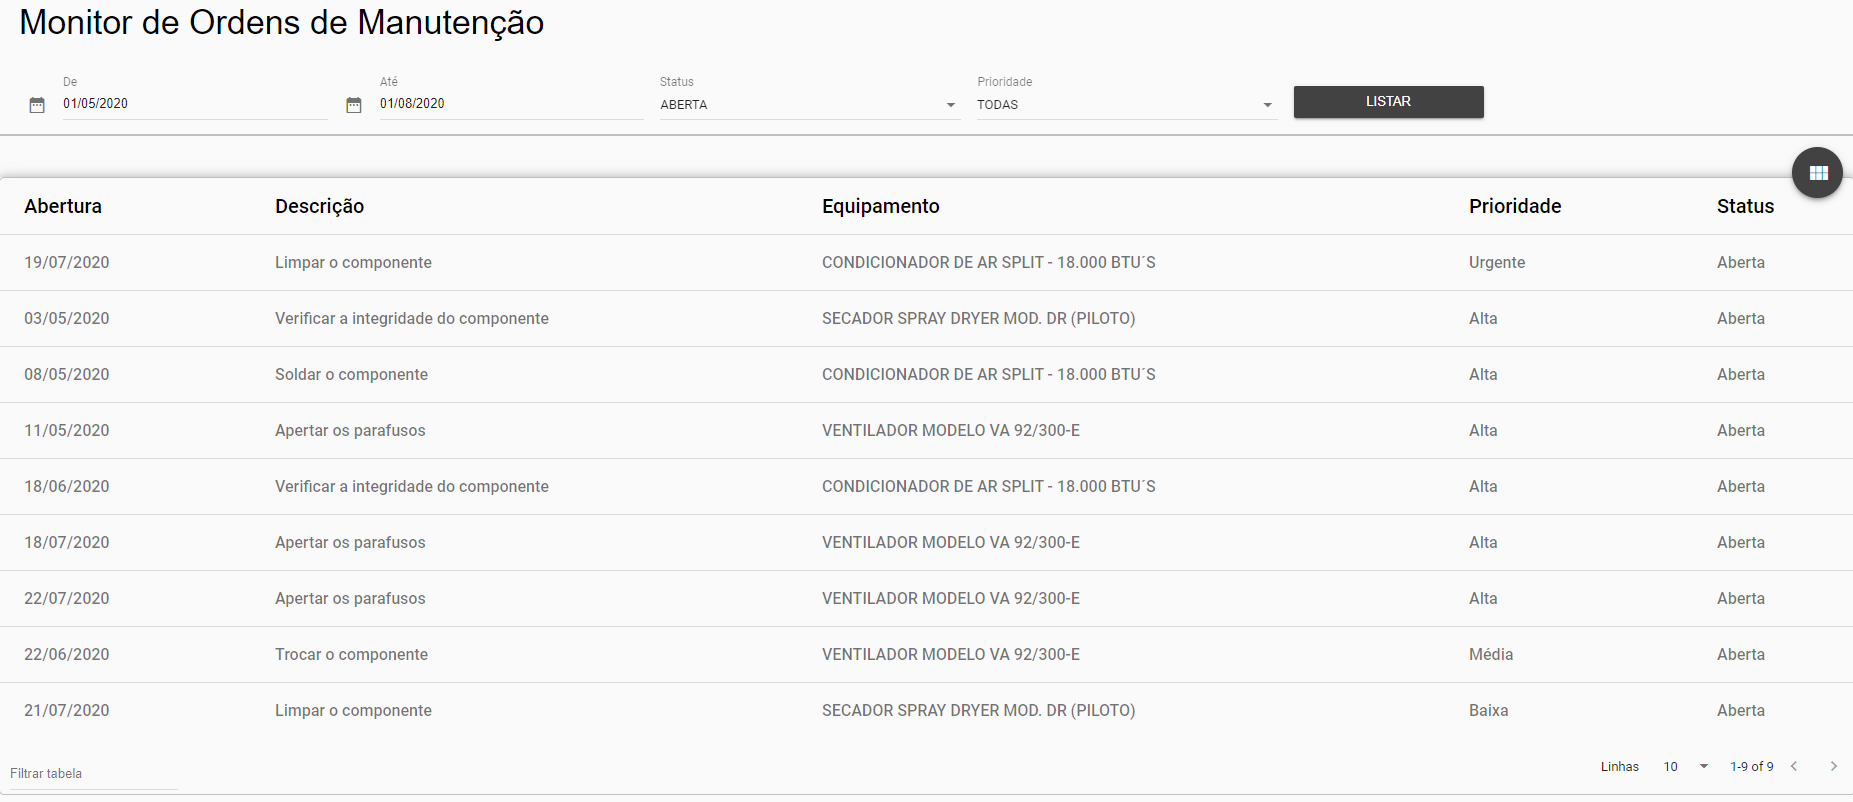
\includegraphics[scale=0.34]{./Figuras/agil.it/web-monitor-lista.png}
	\end{center}
	\legend{Fonte: os autores (2020)}
\end{figure}

\begin{figure}[H]
	\caption{\label{web-monitor-cards}Dashboard: Visualização por cards}
	\begin{center}
		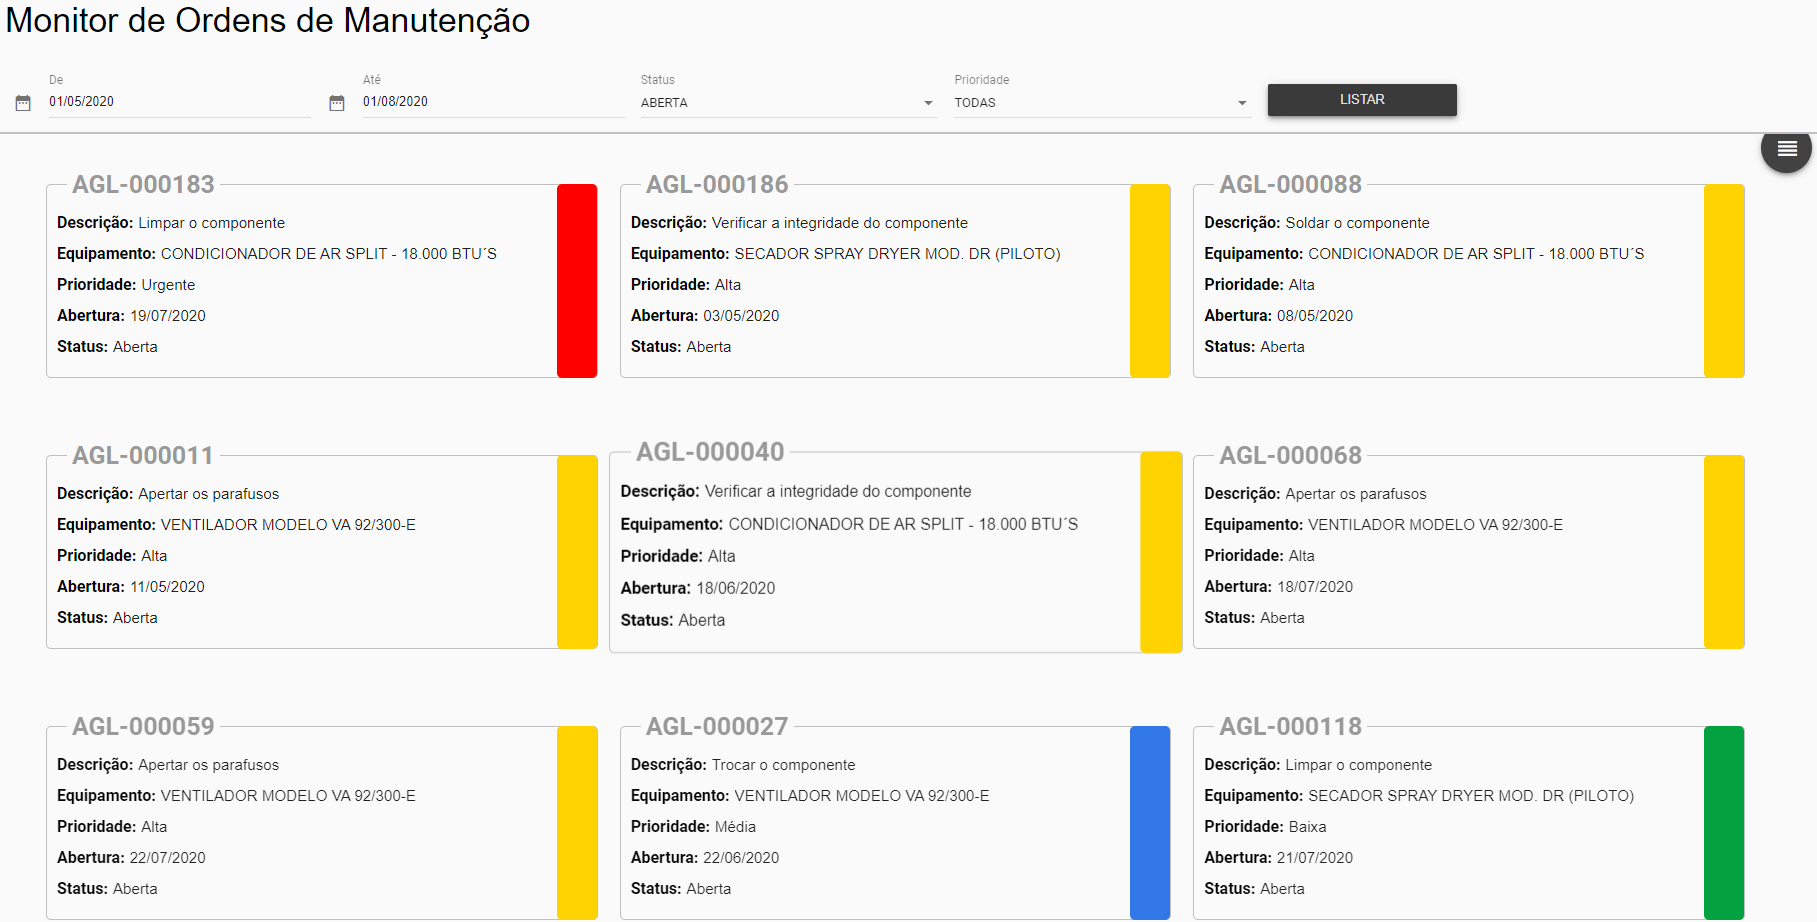
\includegraphics[scale=0.34]{./Figuras/agil.it/web-monitor-cards.png}
	\end{center}
	\legend{Fonte: os autores (2020)}
\end{figure}

\subsection{Análise de Pendências de Assinatura}

\begin{figure}[H]
	\caption{\label{web-pendencias}Análise de pendências de assinatura}
	\begin{center}
		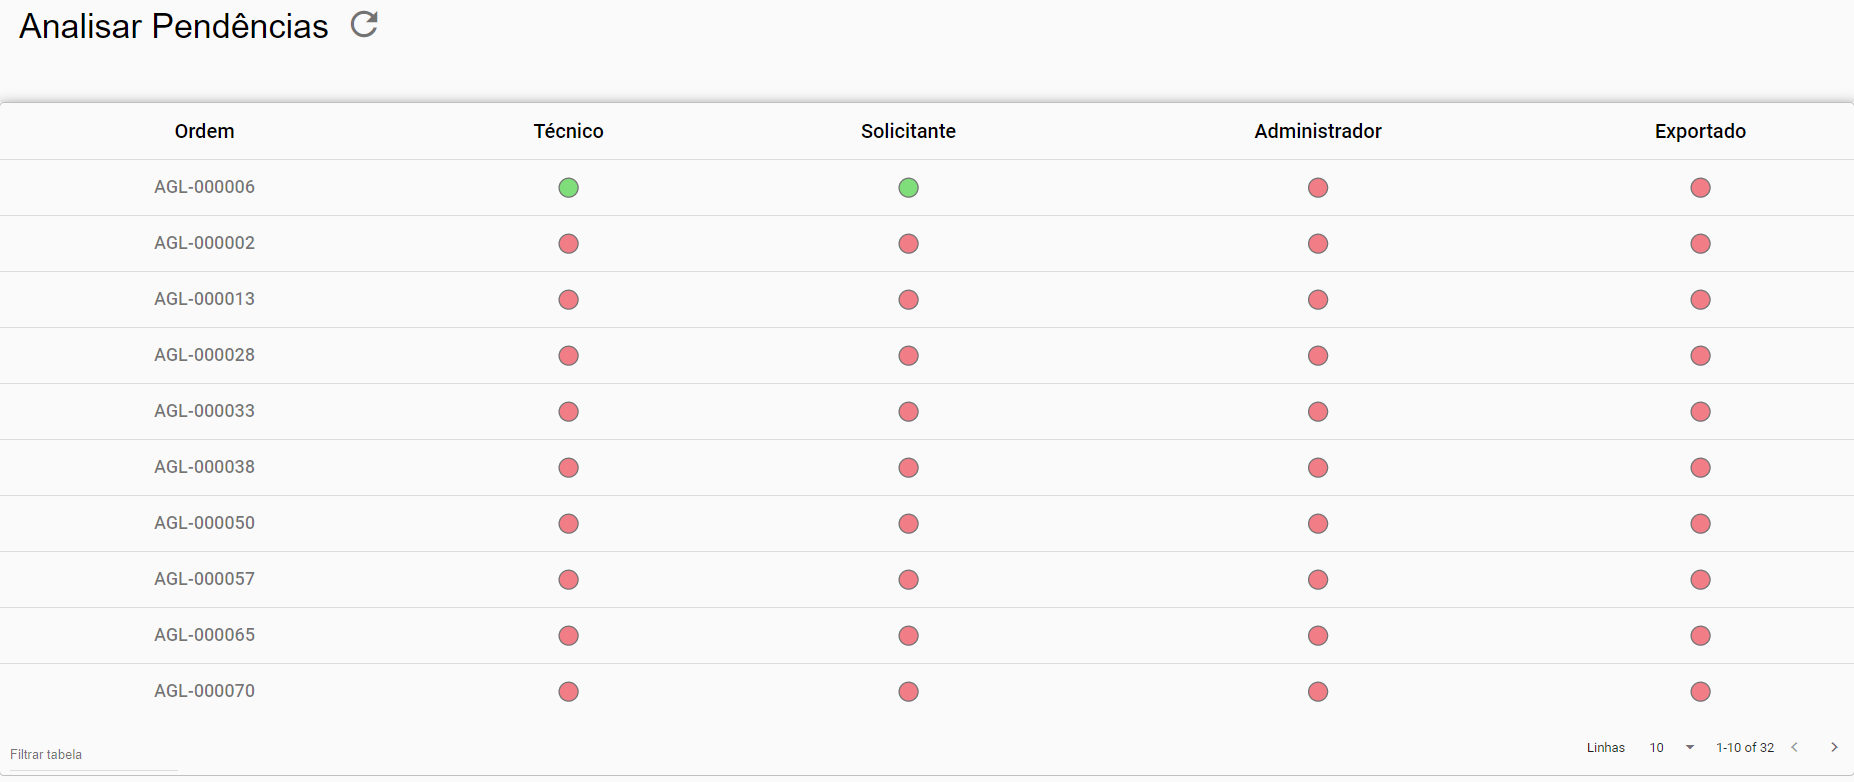
\includegraphics[scale=0.34]{./Figuras/agil.it/web-pendencias.png}
	\end{center}
	\legend{Fonte: os autores (2020)}
\end{figure}

A figura \ref{web-pendencias} mostra a tela de análise de pendências de assinatura que busca de forma automática todas as ordens de manutenção que estão com assinaturas pendentes seja pelo técnico, solicitante ou administrador. Os responsáveis pela ordem que ainda não assinaram são identificados pelo círculo na cor vermelha e os que já assinaram na cor verde. A ordem de manutenção irá permanecer na lista de pendências até ser exportada ao sistema SAP.
Apenas o usuário com o perfil administrador tem acesso a essa tela.

\subsection{Ordem de Manutenção}

\begin{figure}[H]
	\caption{\label{web-om}Ordem de Manutenção}
	\begin{center}
		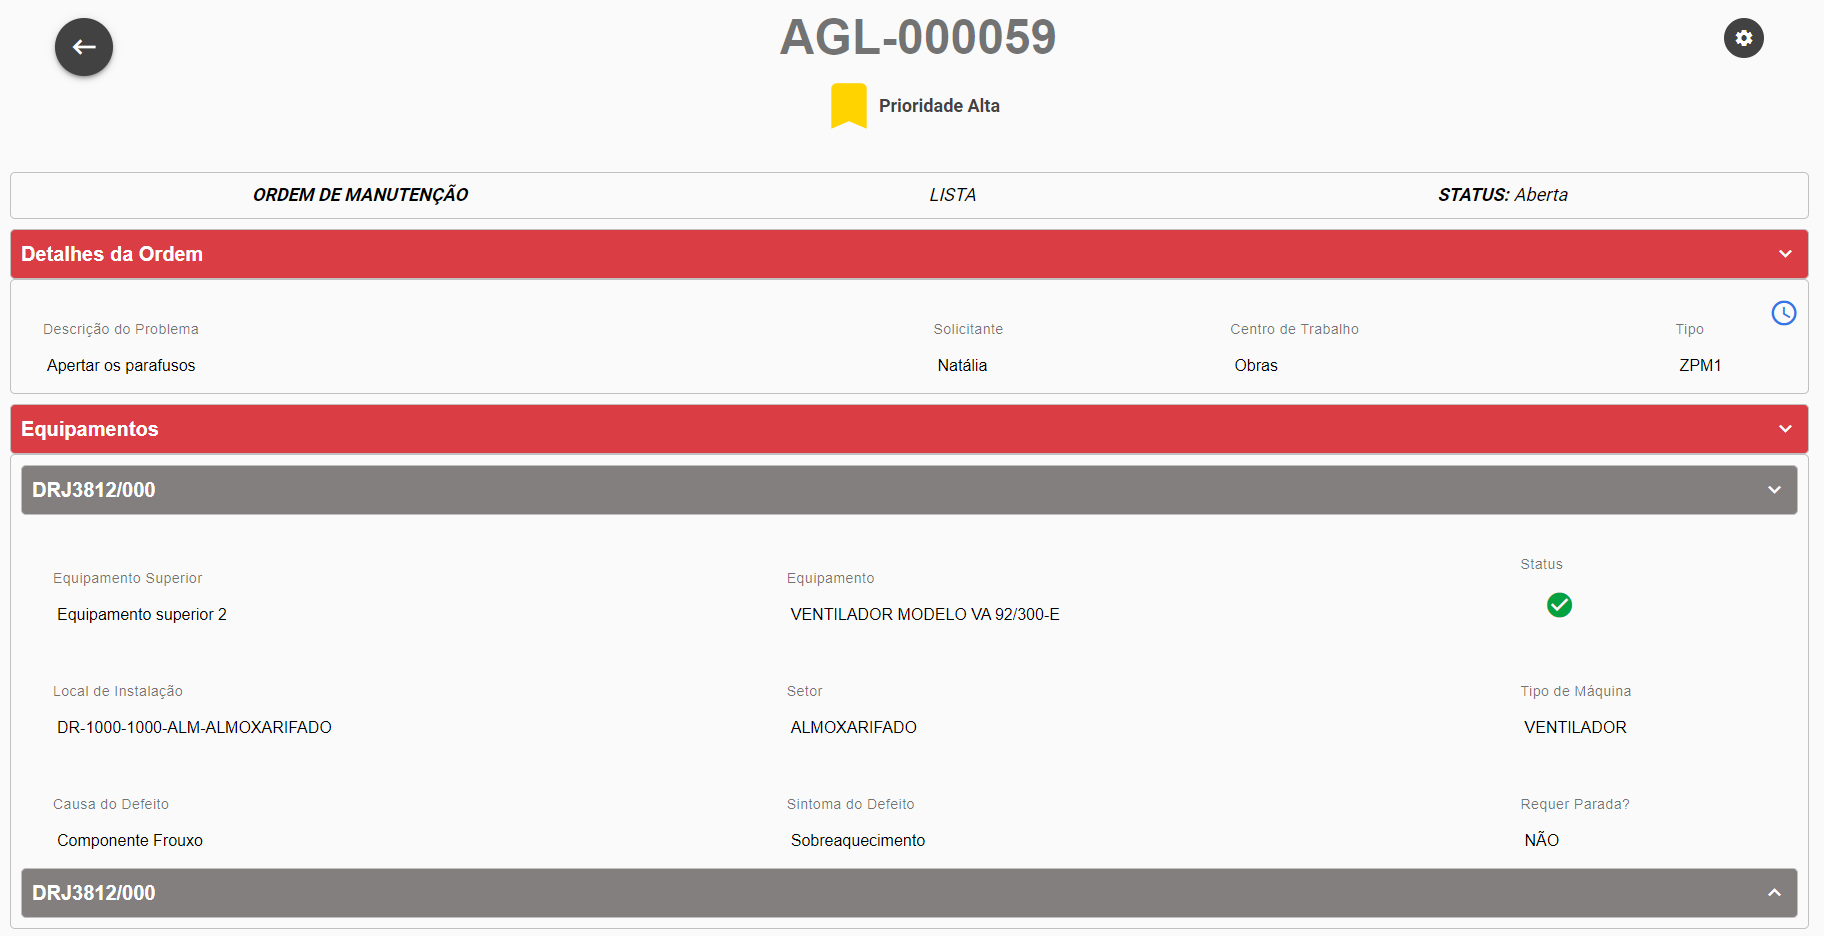
\includegraphics[scale=0.34]{./Figuras/agil.it/web-om.png}
	\end{center}
	\legend{Fonte: os autores (2020)}
\end{figure}

Na figura \ref{web-om} é possível visualizar todas as informações relacionadas a ordem e todas as ações executadas nela, como por exemplo, quem solicitou a abertura de determinada ordem, a data e hora de abertura, todos os equipamentos e operações realizadas em cada um deles. Além disso, no canto superior direito da tela existe um menu com uma série de ações, onde se encontra a opção para efetuar a assinatura da ordem de manutenção, a parte mais importante no fluxo do processo. Para solicitar a assinatura é necessário informar a senha do usuário logado e concordar com todas as informações existentes na ordem, com isso, os dados são enviados e analisados pelo servidor que retorna uma mensagem de sucesso ou erro de acordo com a análise feita, conforme mostra a figura \ref{web-assinatura}.

\begin{figure}[H]
	\caption{\label{web-assinatura}Assinatura da Ordem de Manutenção}
	\begin{center}
		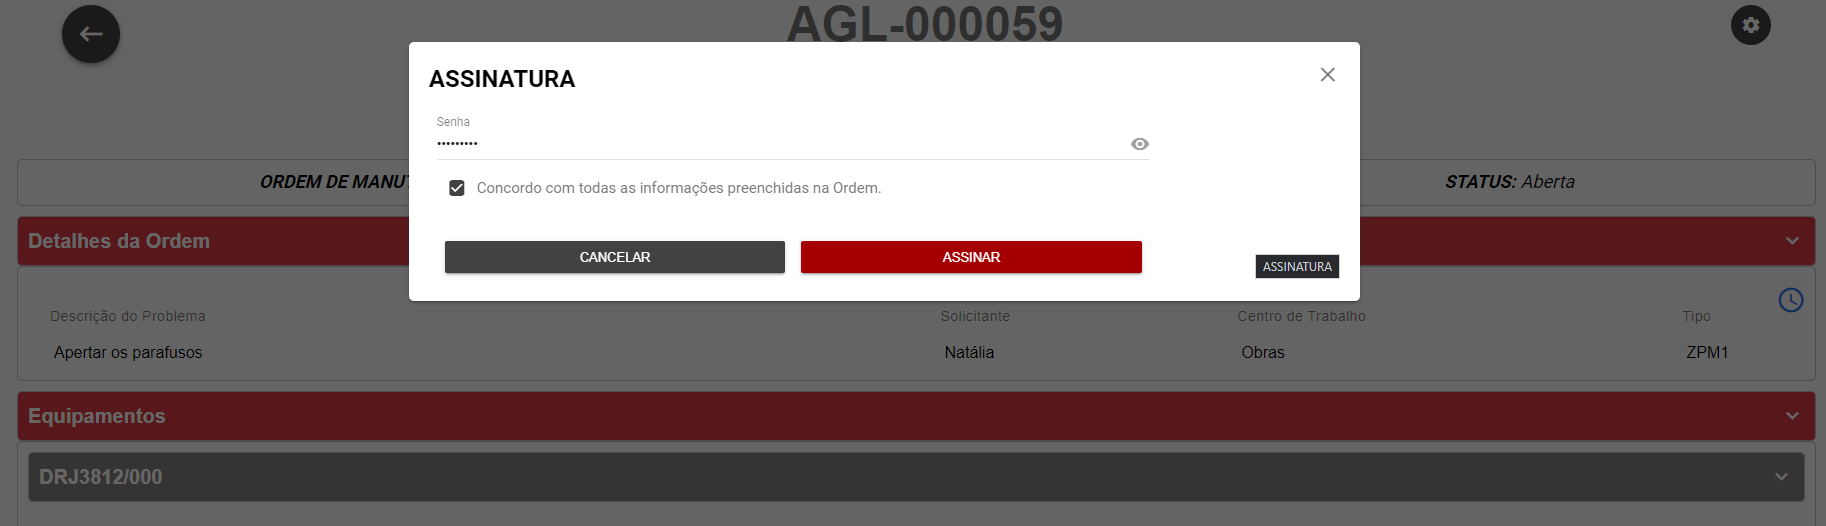
\includegraphics[scale=0.32]{./Figuras/agil.it/web-assinatura.png}
	\end{center}
	\legend{Fonte: os autores (2020)}
\end{figure}

\section{Mobile}
O aplicativo mobile será de suma importância para a execução das ordens de manutenção por parte dos técnicos, nele poderá ser executado todas as ações no que diz respeito às ordens de manutenção. A facilidade de uso possibilita a execução de ordens de manutenção com maior agilidade e eficiência.

\subsection{Monitor de Ordens de Manutenção}
\begin{figure}[H]
	\caption{\label{mobile-monitor}Monitor de Ordens de Manutenção}
	\begin{center}
		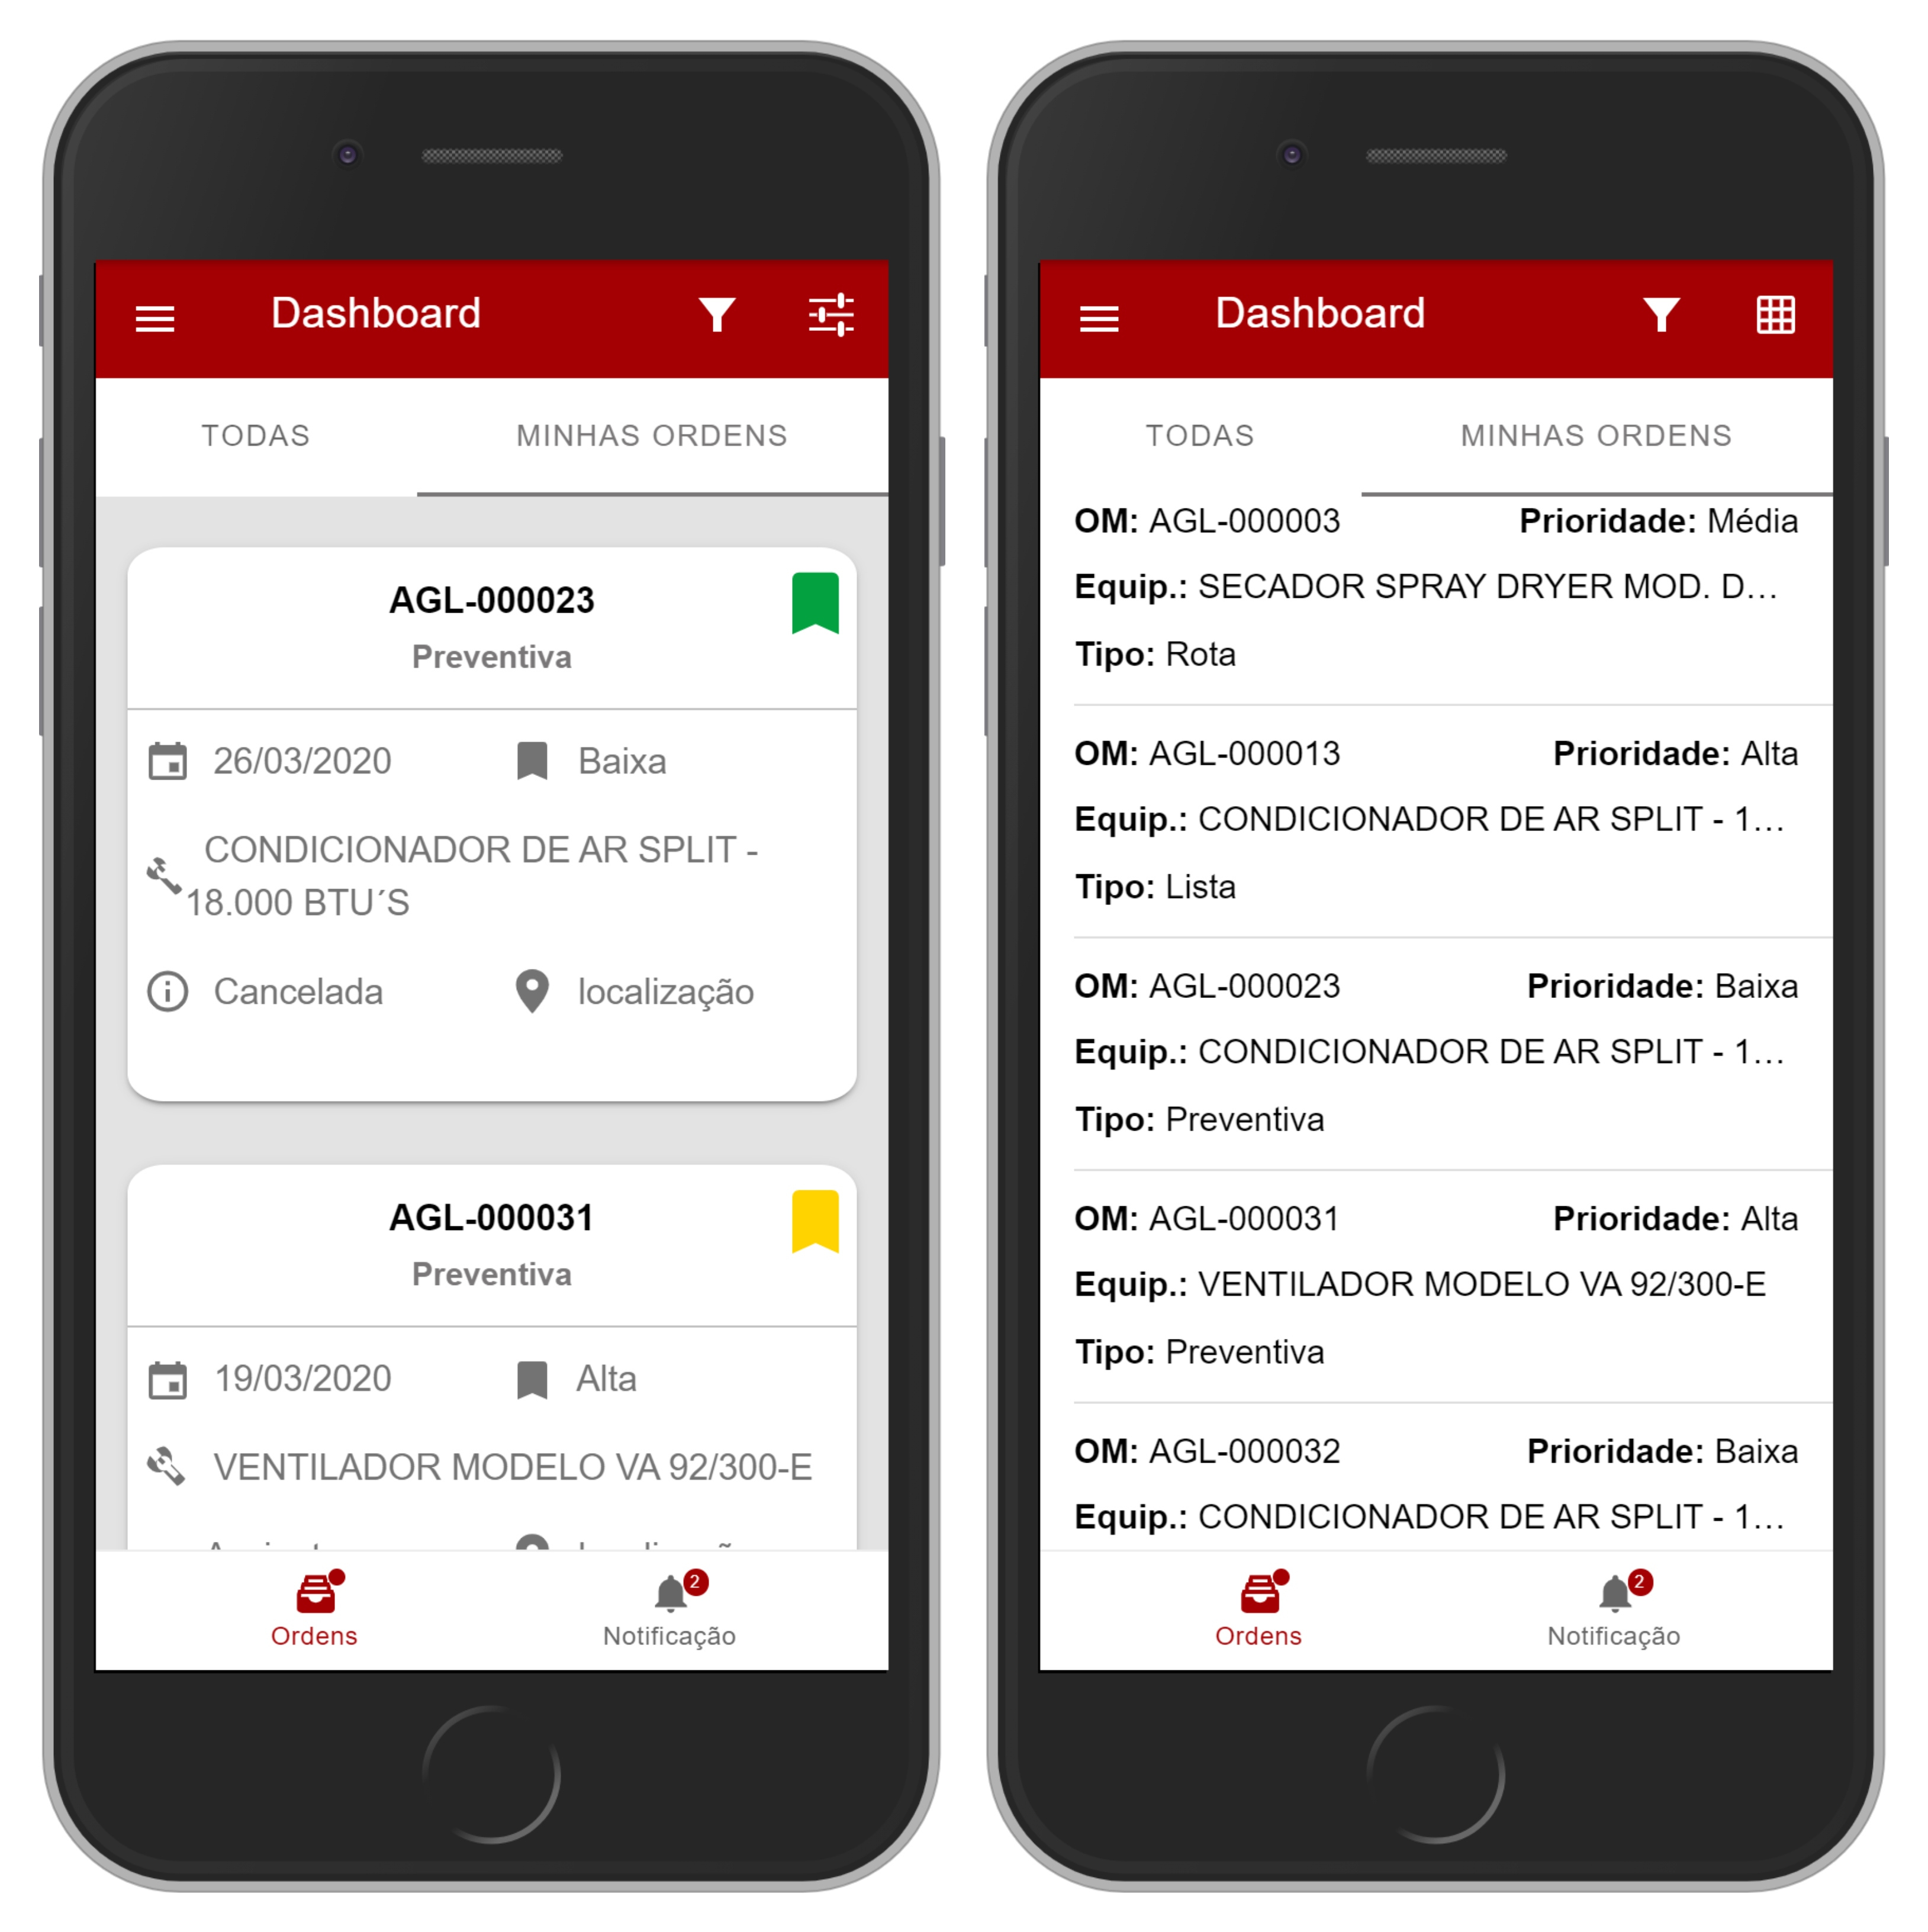
\includegraphics[scale=0.55]{./Figuras/agil.it/mobile-monitor.jpg}
	\end{center}
	\legend{Fonte: os autores (2020)}
\end{figure}

A figura \ref{mobile-monitor} mostra o monitor que os técnicos irão utilizar, ele tem duas visualizações: Cards e Lista, e separa as ordens em duas abas: Todas e Minhas Ordens para que o técnico possa rapidamente verificar em quais ordens ele está envolvido.

O monitor também possui filtros para facilitar a busca de Ordens de manutenção, conforme mostra a figura \ref{mobile-monitor-filtro}
\begin{figure}[H]
	\caption{\label{mobile-monitor-filtro}Filtros do Monitor}
	\begin{center}
		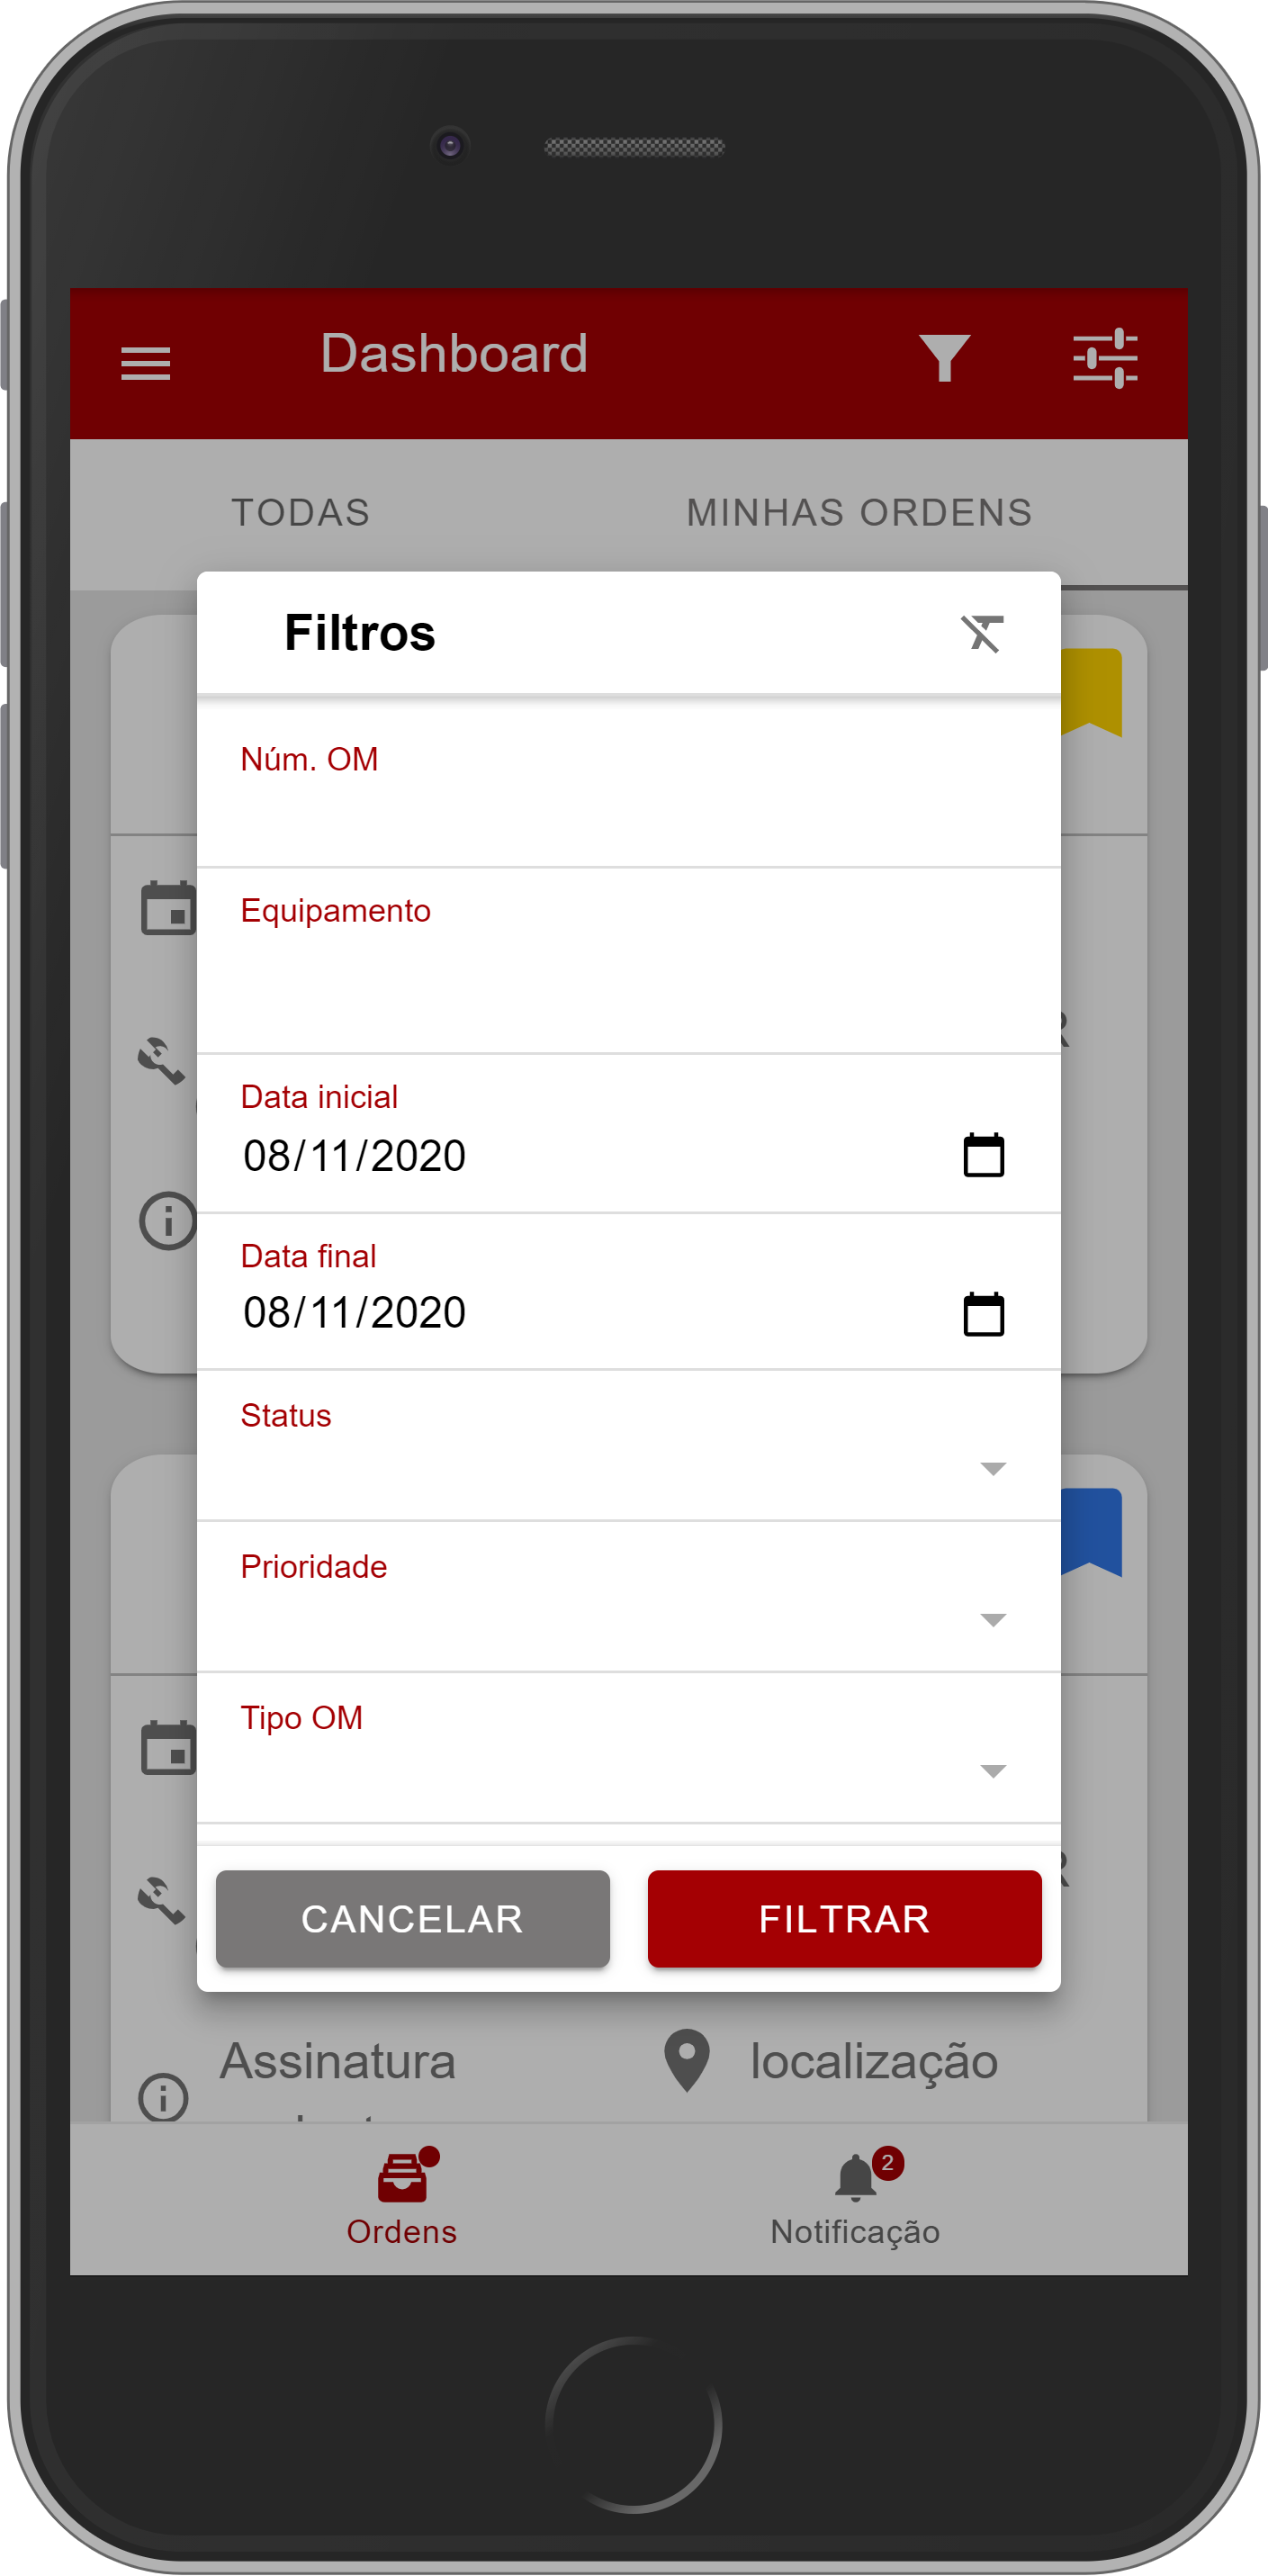
\includegraphics[scale=0.20]{./Figuras/agil.it/mobile-monitor-filtro.png}
	\end{center}
	\legend{Fonte: os autores (2020)}
\end{figure}
Por padrão, o monitor não apresenta ordens que estão nas situações finais: finalizada ou cancelada, só serão exibidas se forem informados explicitamente nos filtros.

\subsection{Ordem de Manutenção Corretiva/Preventiva}

\begin{figure}[H]
	\caption{\label{mobile-om-preventiva}Ordem de Manutenção Corretiva/Preventiva}
	\begin{center}
		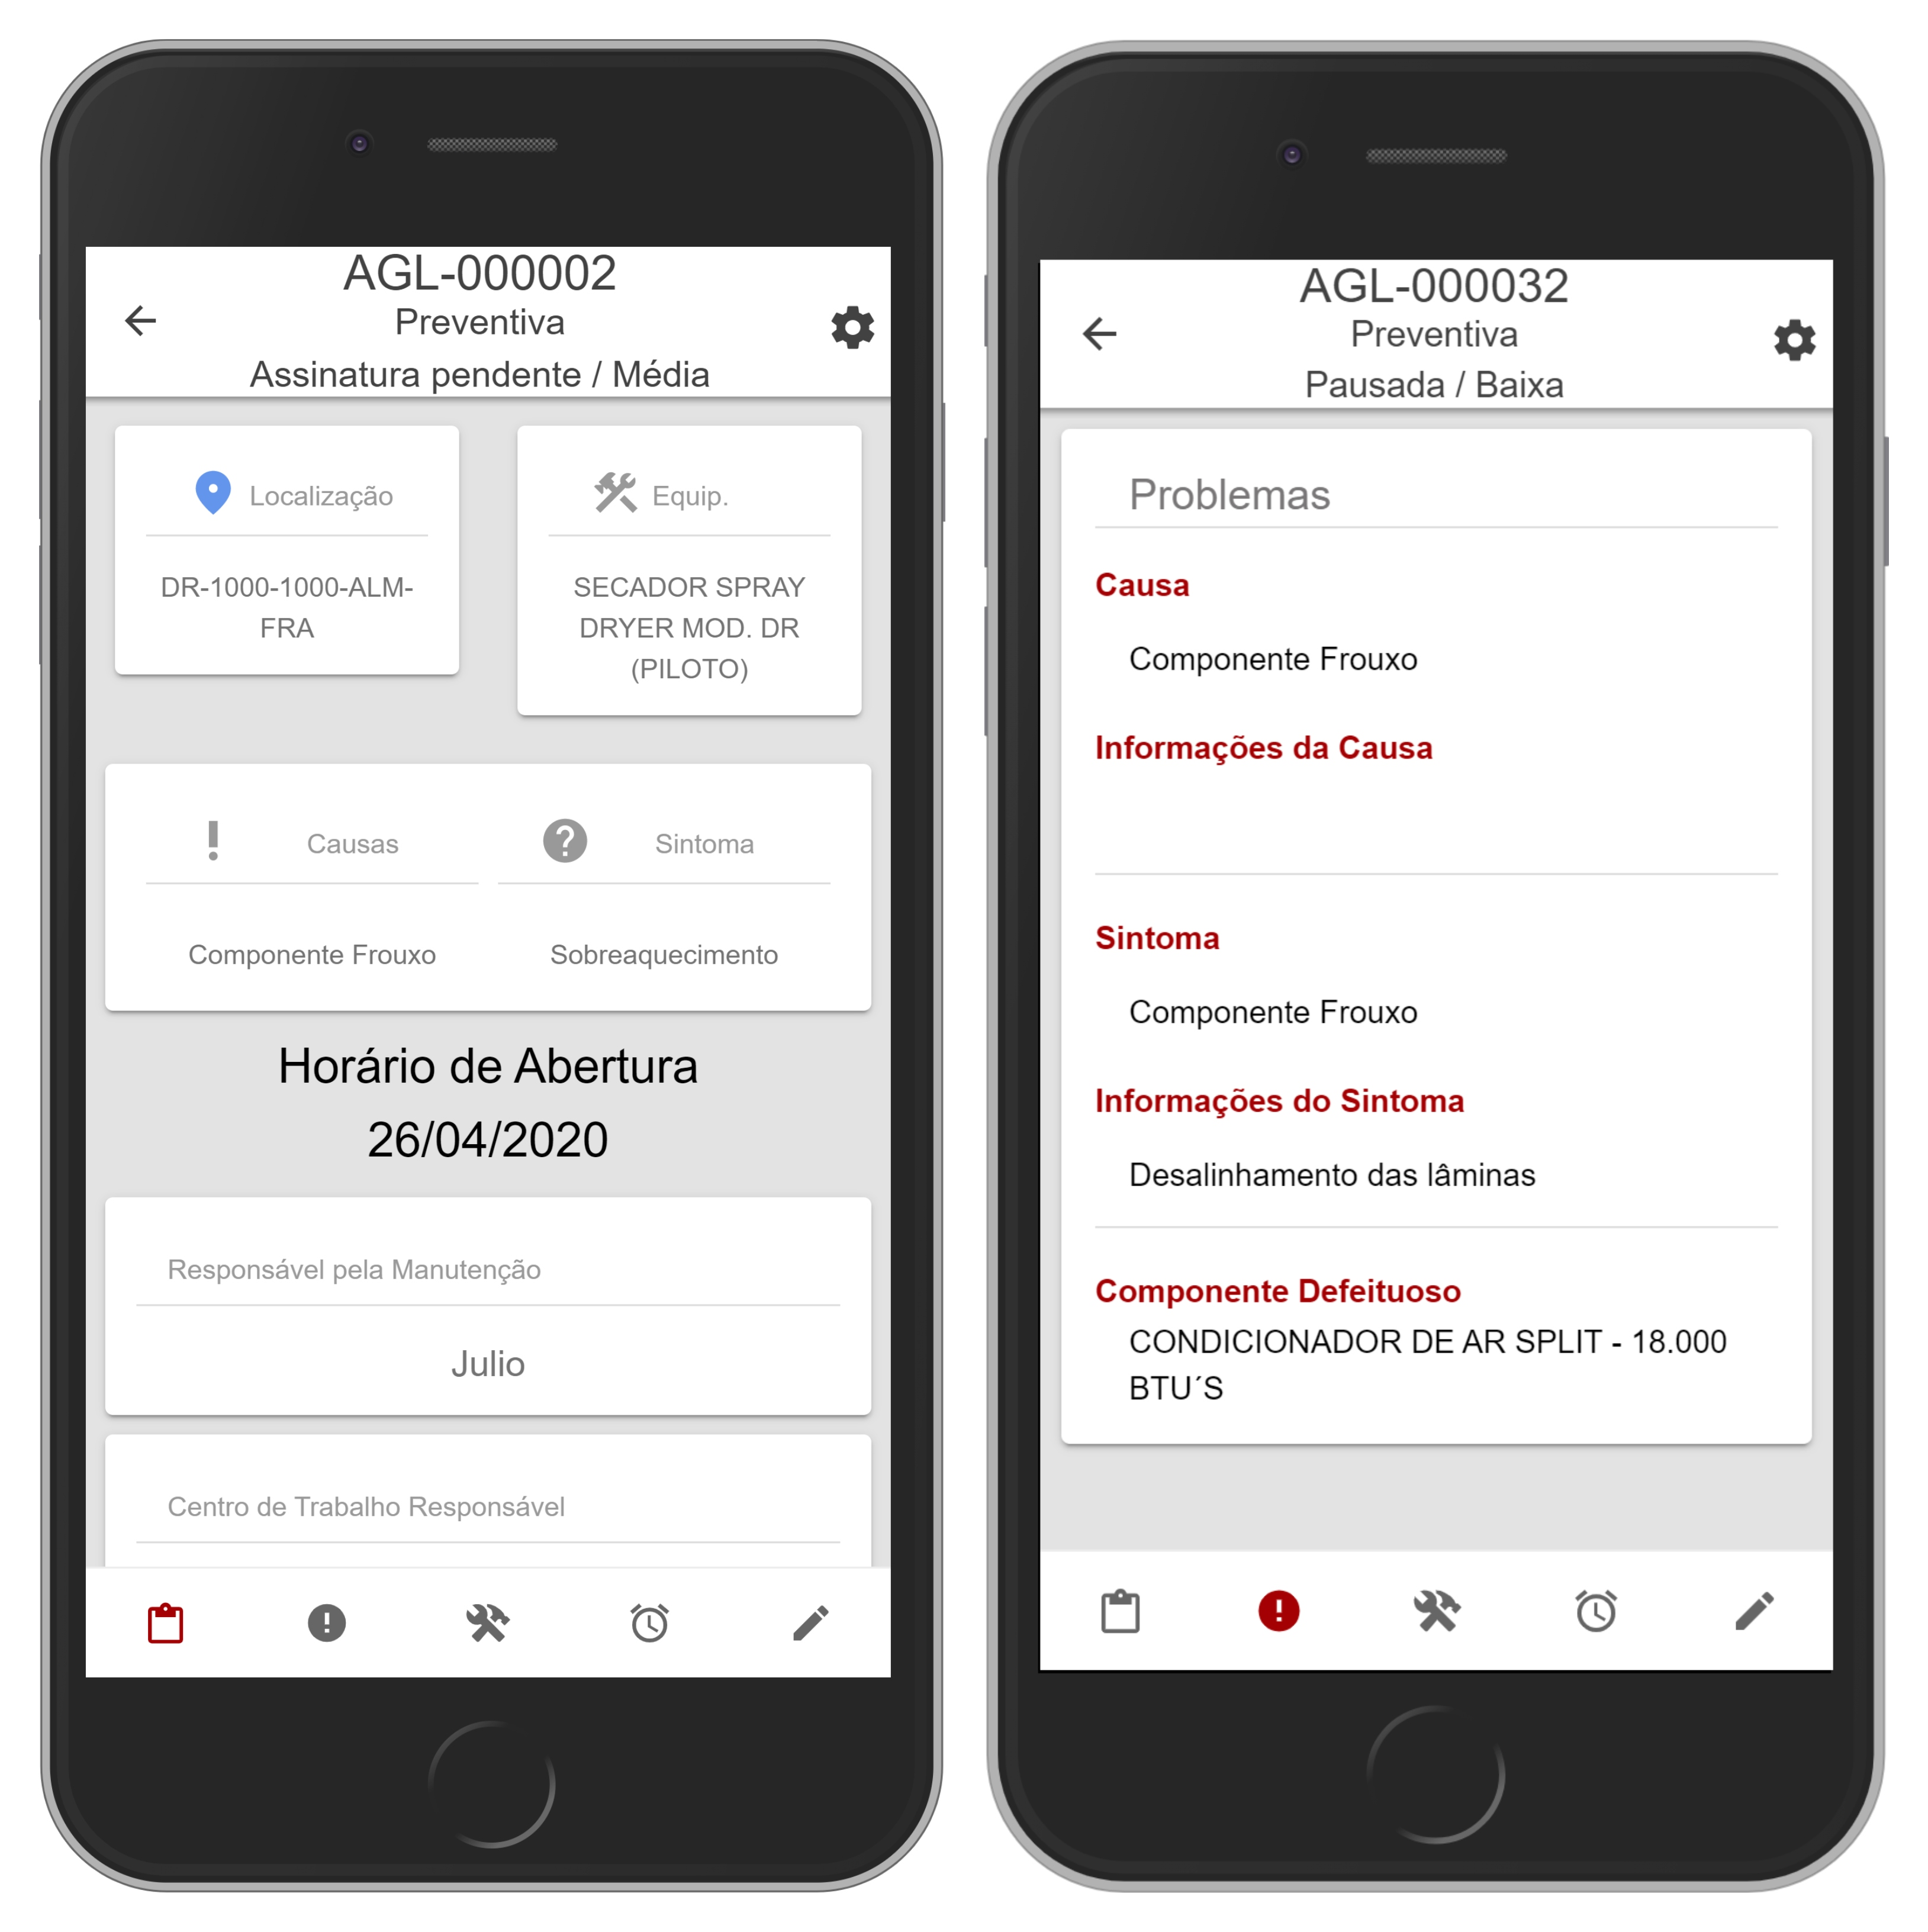
\includegraphics[scale=0.55]{./Figuras/agil.it/mobile-om-preventiva.jpg}
	\end{center}
	\legend{Fonte: os autores (2020)}
\end{figure}

A figura \ref{mobile-om-preventiva} mostra o detalhamento das duas primeiras abas da ordem do \textit{layout} corretiva/preventiva, a primeira aba mostra dados pertinentes ao técnico como o equipamento e a localização do mesmo, a causa e o sintoma do problema. Na segunda aba é um detalhamento mais aprofundado do problema identificado, mostrando a causa, sintoma e o componente defeituoso. A terceira aba é de operações, a quarta de apontamentos e a quinta de assinaturas, todas serão abordadas a seguir.

\subsection{Ordem de Manutenção Lista e Rota}

\begin{figure}[H]
	\caption{\label{mobile-om-rota}Ordem de Manutenção Lista e Rota}
	\begin{center}
		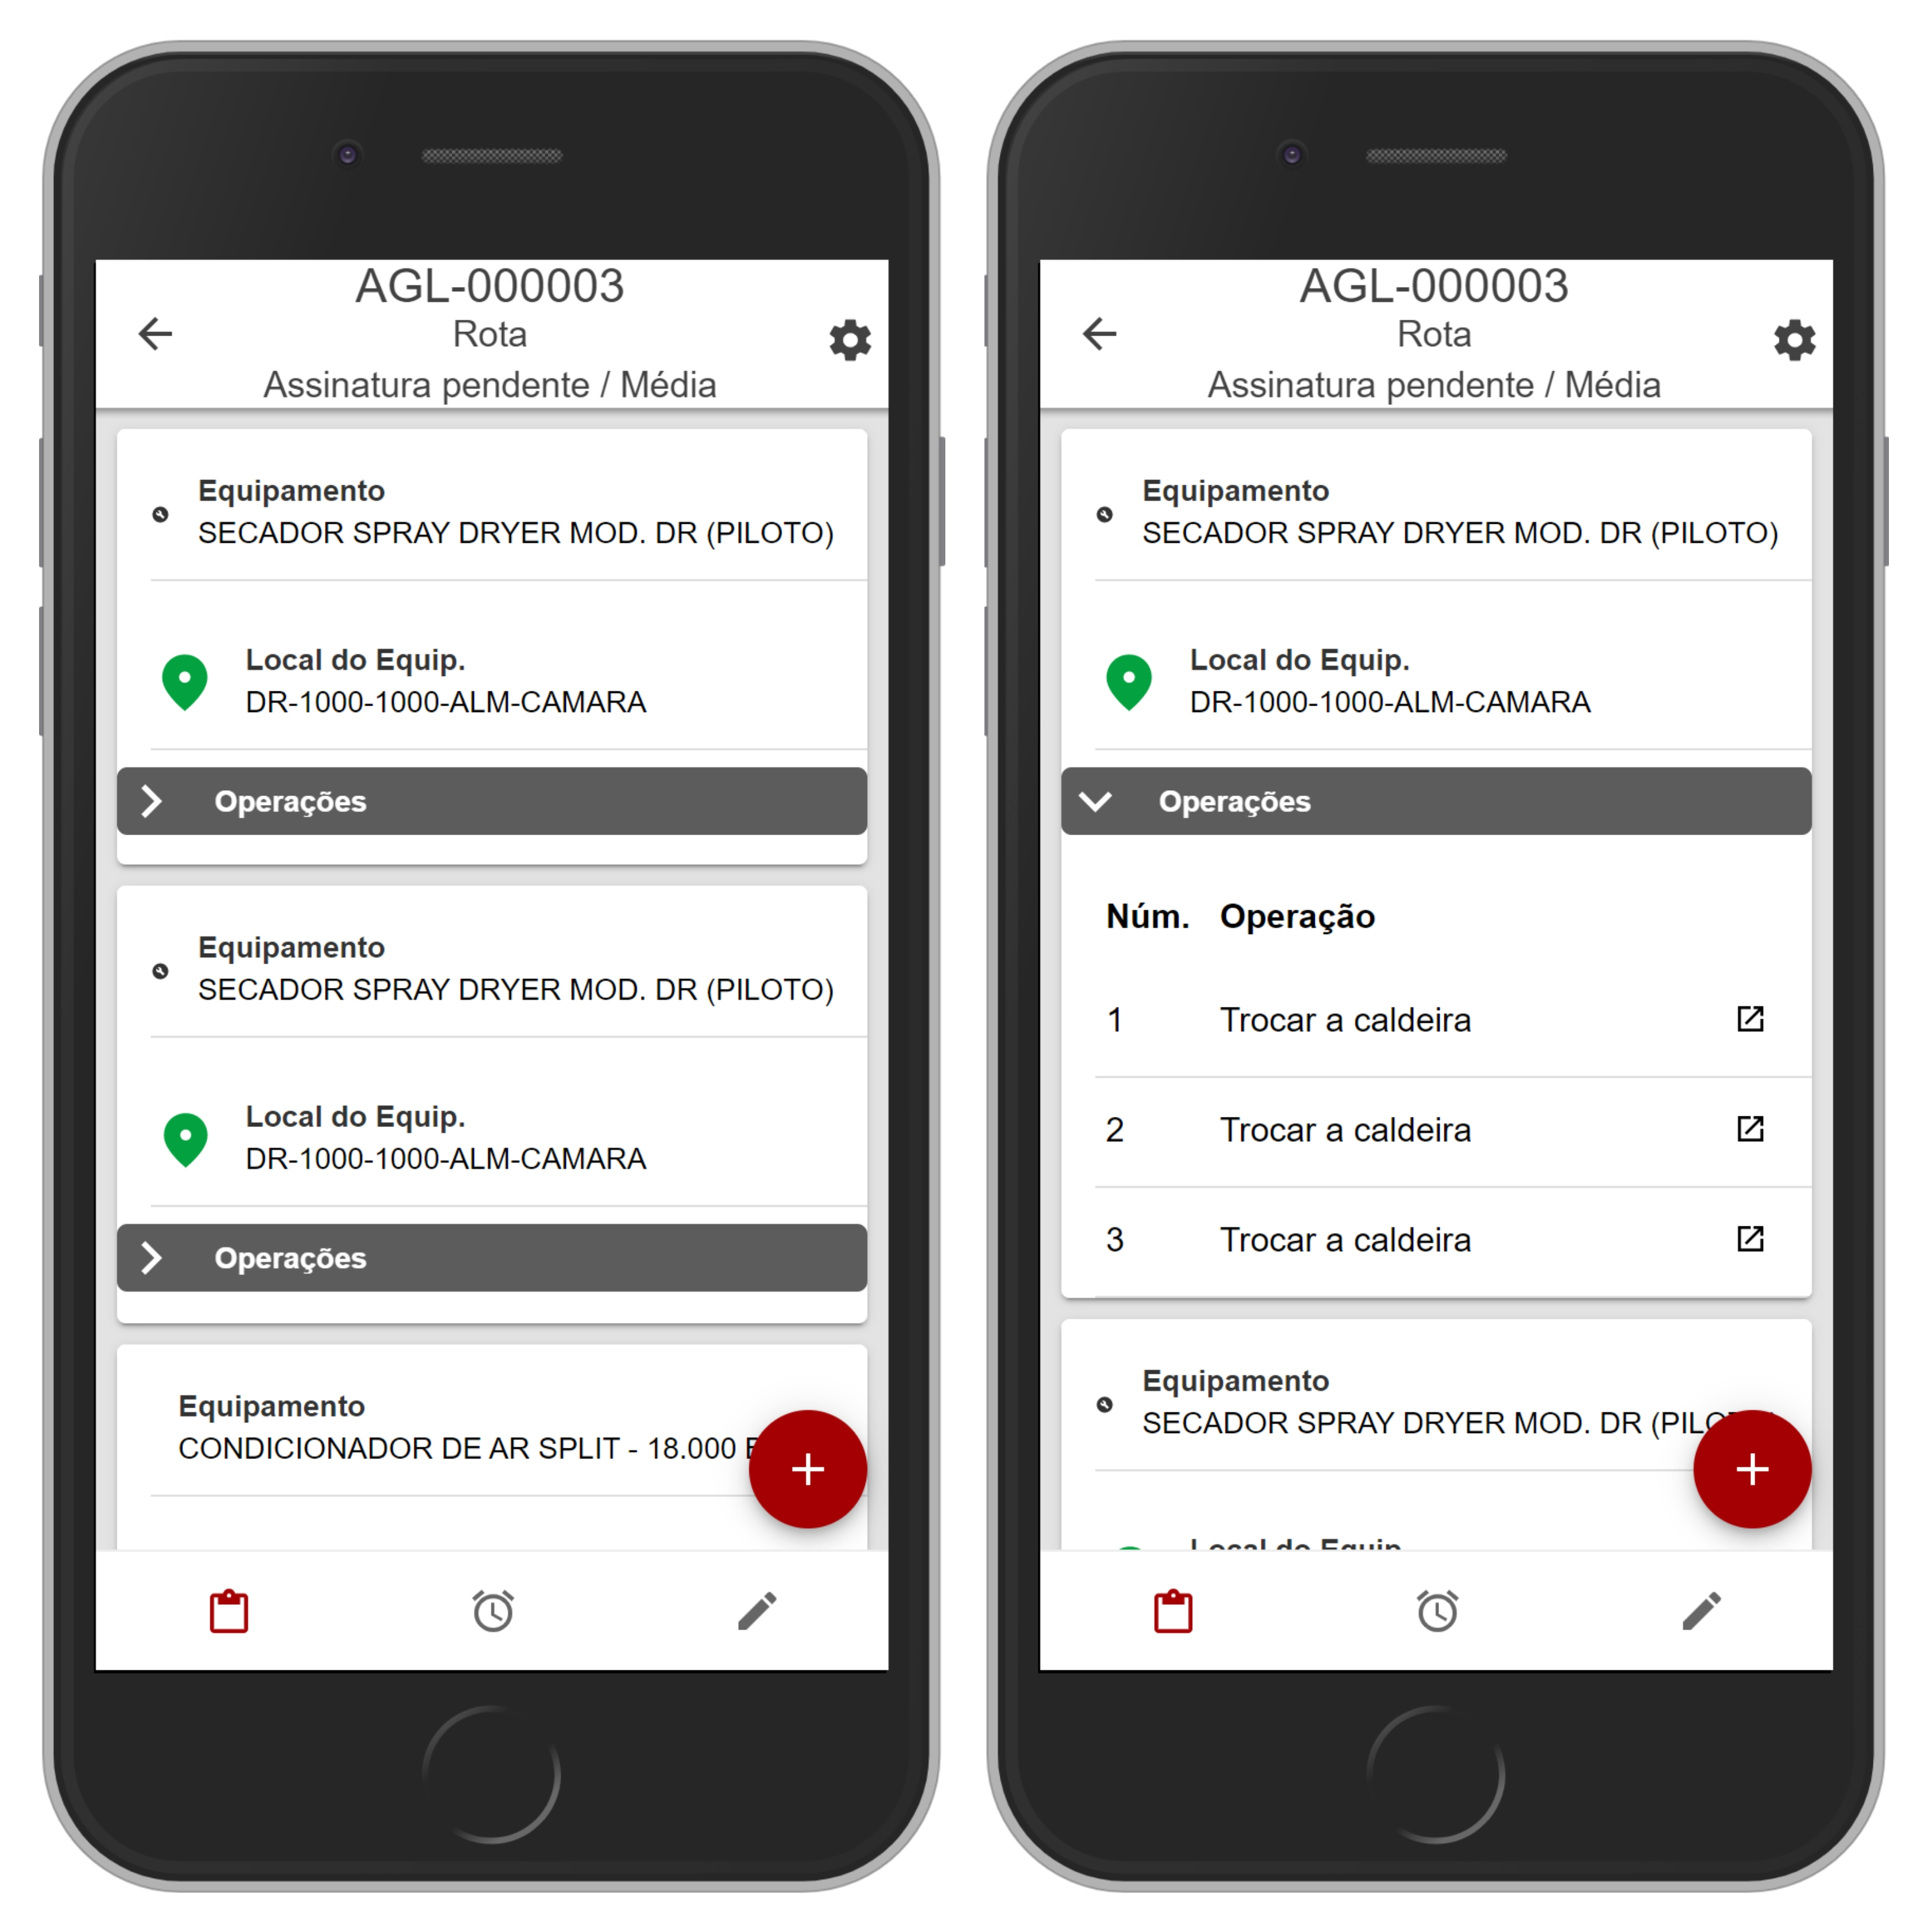
\includegraphics[scale=0.55]{./Figuras/agil.it/mobile-om-rota.jpg}
	\end{center}
	\legend{Fonte: os autores (2020)}
\end{figure}

A figura \ref{mobile-om-rota} mostra o detalhamento da primeira aba da ordem dos \textit{layouts} lista e rota que é a aba de operações. Nela, tem uma listagem de todos os equipamentos da ordem e suas operações. O técnico pode criar novas operações clicando no botão de ``+'' ou detalhar/editar uma operação clicando na linha dela.
A segunda aba é de apontamentos e a terceira de assinatura, que serão abordadas posteriormente.

\subsection{Operações da Ordem de Manutenção}

\begin{figure}[H]
	\caption{\label{mobile-om-operacao}Ordem de Manutenção Lista e Rota}
	\begin{center}
		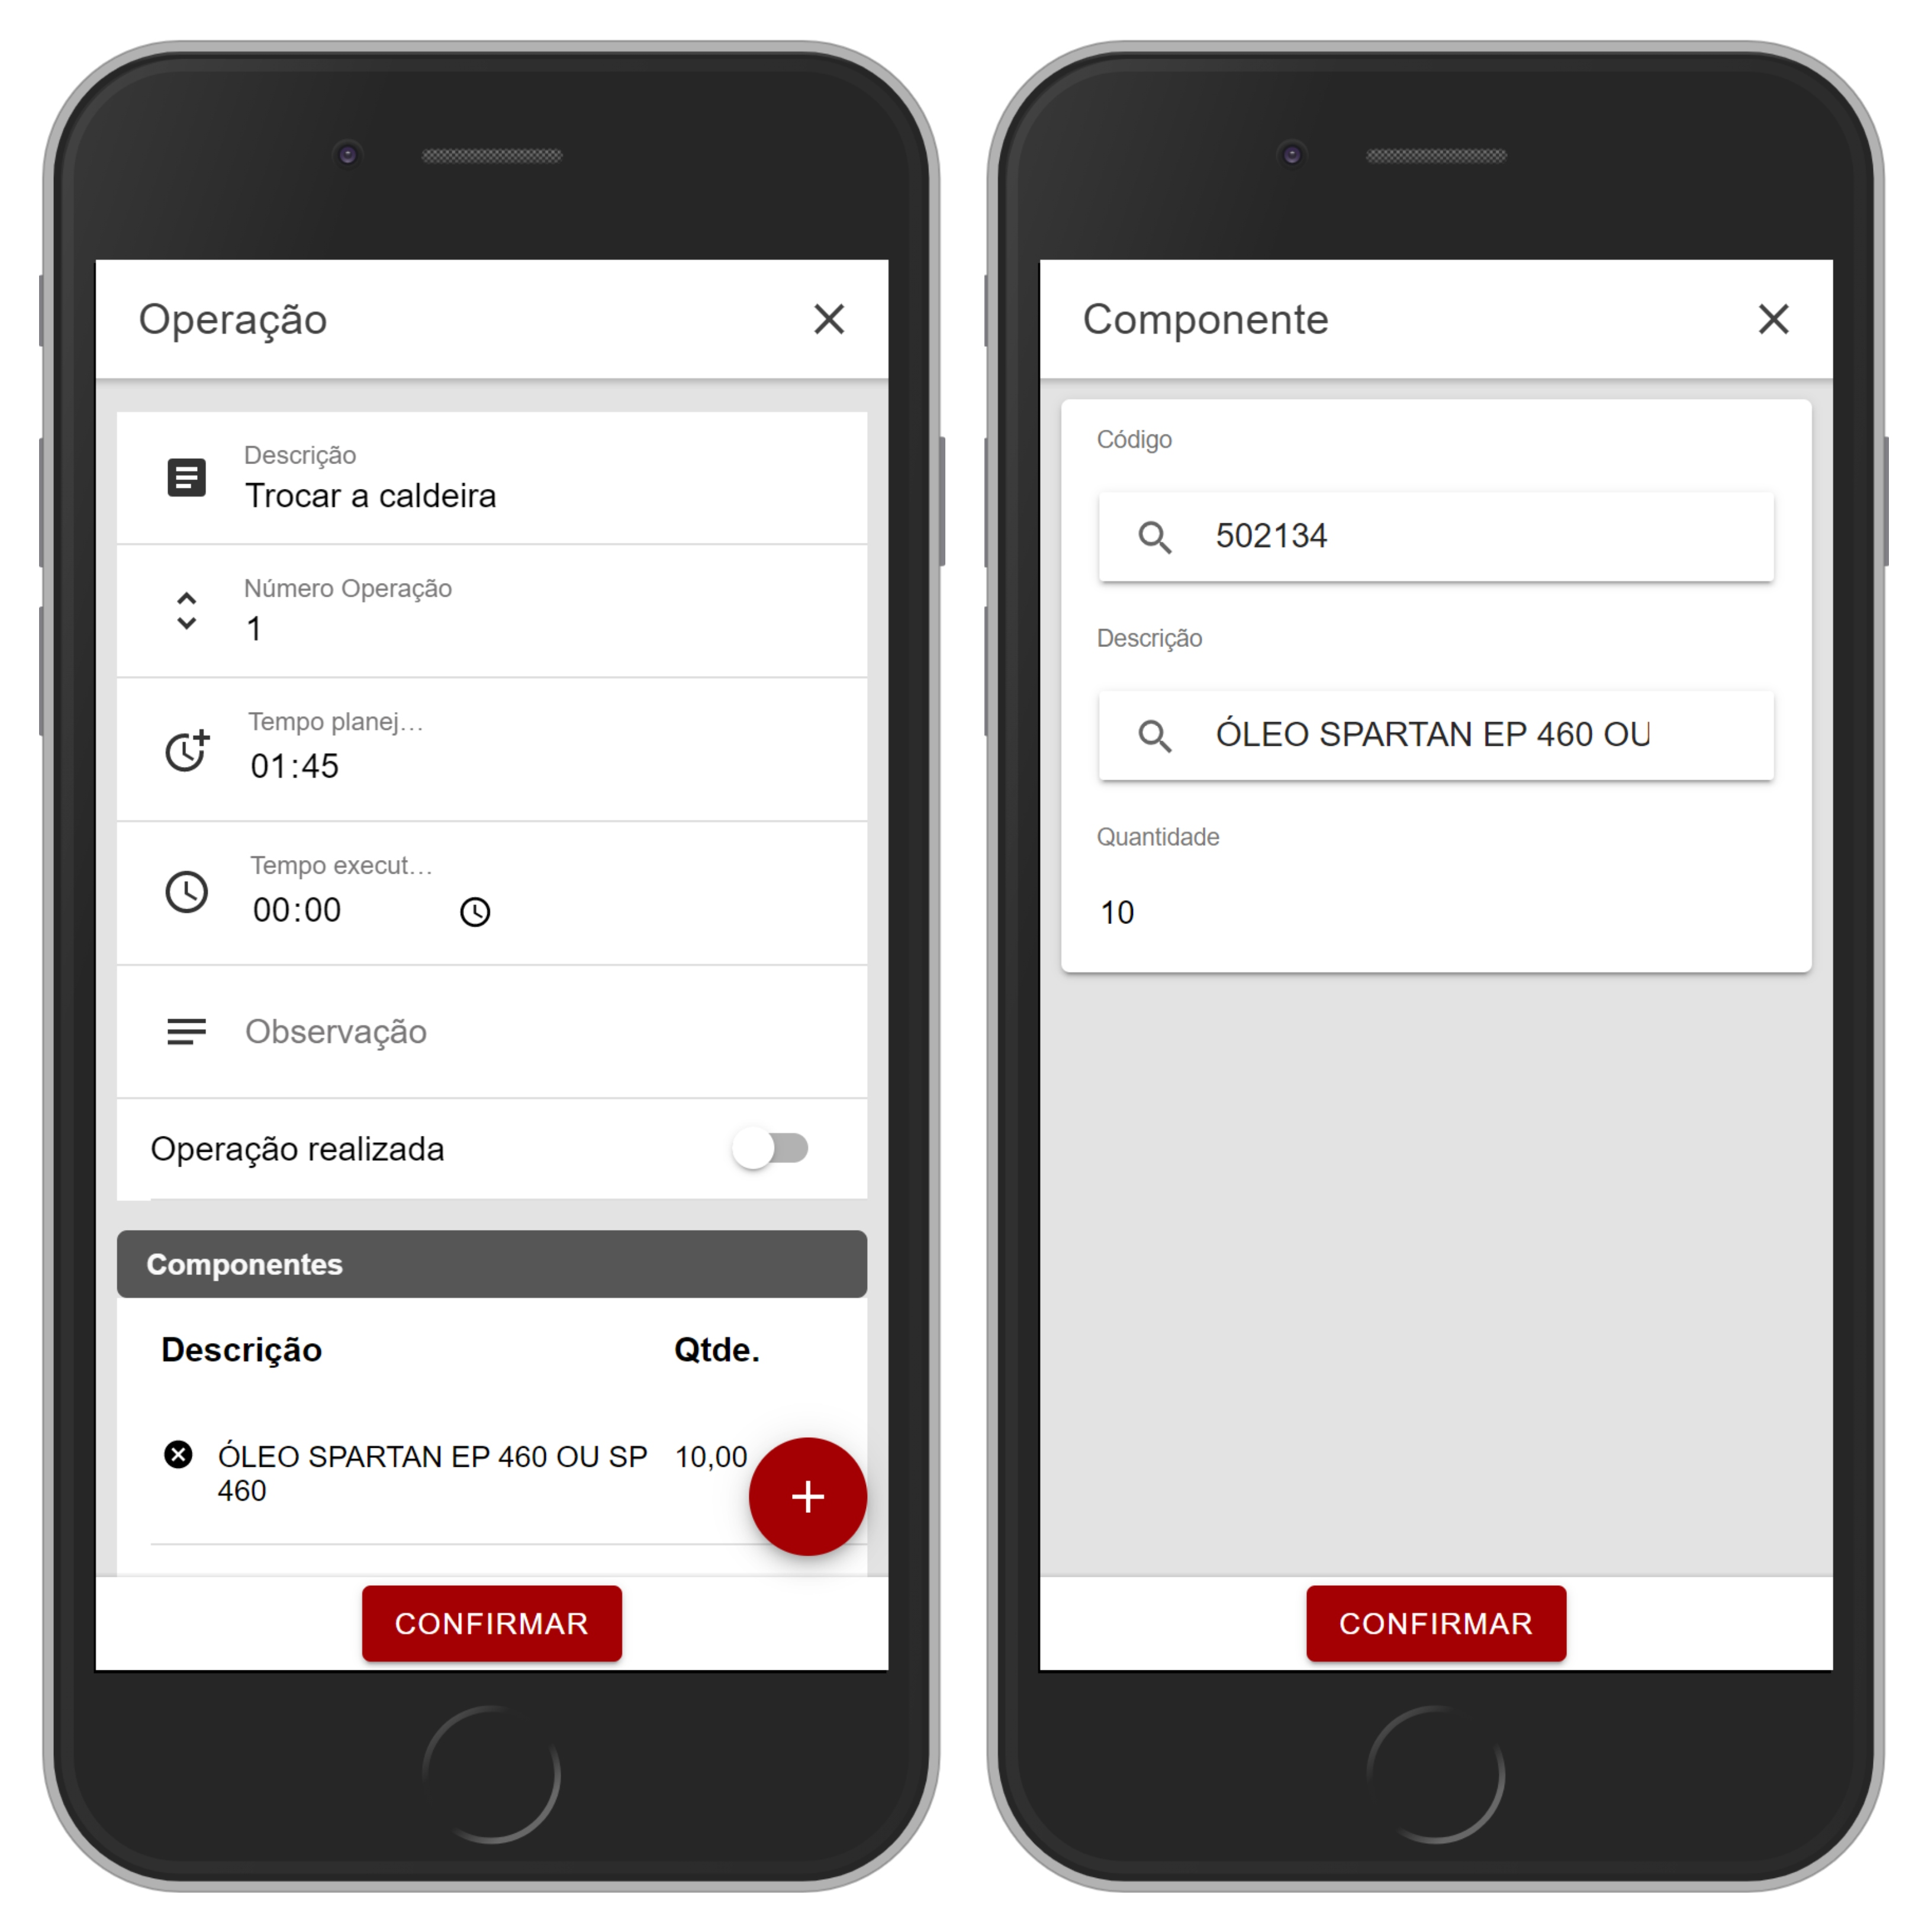
\includegraphics[scale=0.55]{./Figuras/agil.it/mobile-om-operacao.jpg}
	\end{center}
	\legend{Fonte: os autores (2020)}
\end{figure}

Ao clicar em uma operação será aberto a tela mostrada na figura \ref{mobile-om-operacao}, nela é possível colocar o tempo investido em sua execução, se ela já foi executada e adicionar alguma observação, caso necessário.
Para executar determinadas operação, o técnico pode necessitar de alguns insumos, para tanto ele pode adicionar componentes utilizados na operação clicando no botão de ``+'', editar clicando na linha do componente e excluir clicando no ``x'' na primeira coluna da linha.
Para adicionar um novo componente, o técnico pode pesquisar por código ou descrição e deve informar a quantidade utilizada.

\subsection{Apontamento}

\begin{figure}[H]
	\caption{\label{mobile-om-apontamento}Ordem de Manutenção: Apontamento}
	\begin{center}
		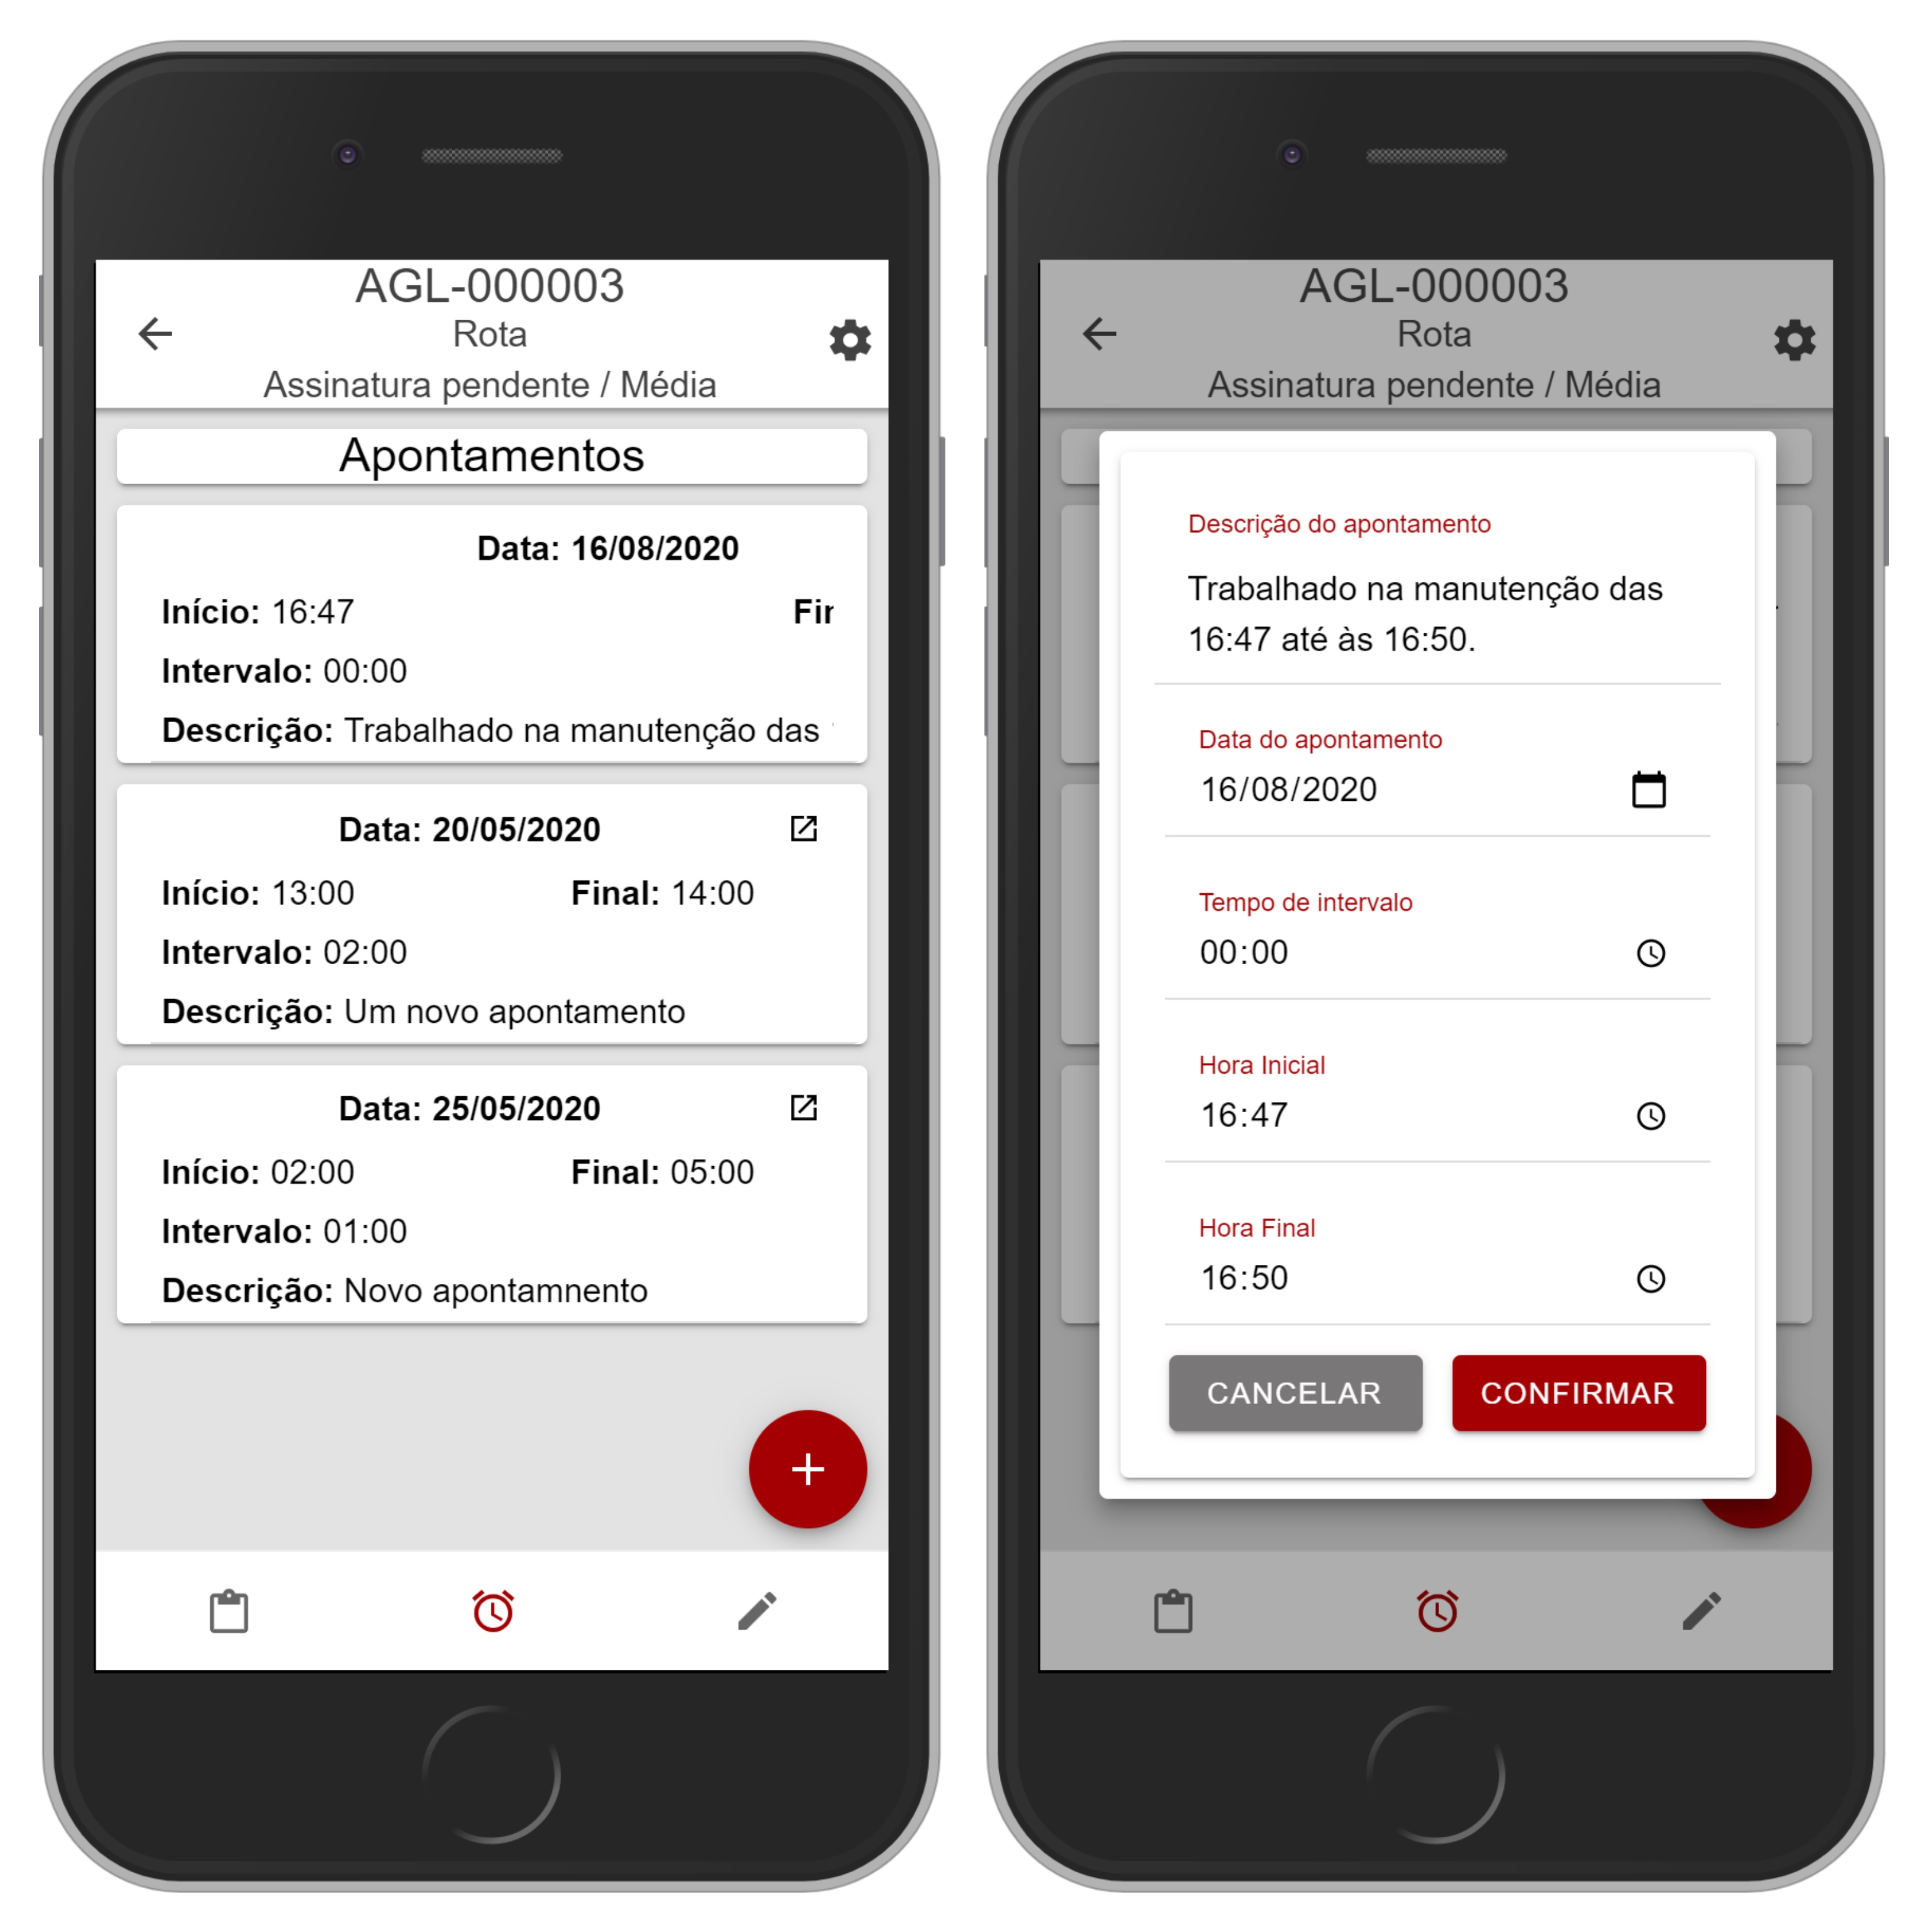
\includegraphics[scale=0.55]{./Figuras/agil.it/mobile-om-apontamento.jpg}
	\end{center}
	\legend{Fonte: os autores (2020)}
\end{figure}

A figura \ref{mobile-om-apontamento} mostra a listagem de apontamentos da OM, nele pode-se editar, excluir e criar um novo apontamento. Ao cadastrar ou editar um registro, o técnico deve informar uma descrição e a data do apontamento, a hora inicial e final. Caso tenha tido algum intervalo, por exemplo almoço, pode-se computar o intervalo no campo tempo de intervalo. Um técnico não pode visualizar apontamentos de outros técnicos na mesma ordem, nem realizar os apontamentos por outro técnico.

\subsection{Assinatura}

\begin{figure}[H]
	\caption{\label{mobile-om-assinatura}Ordem de Manutenção: Apontamento}
	\begin{center}
		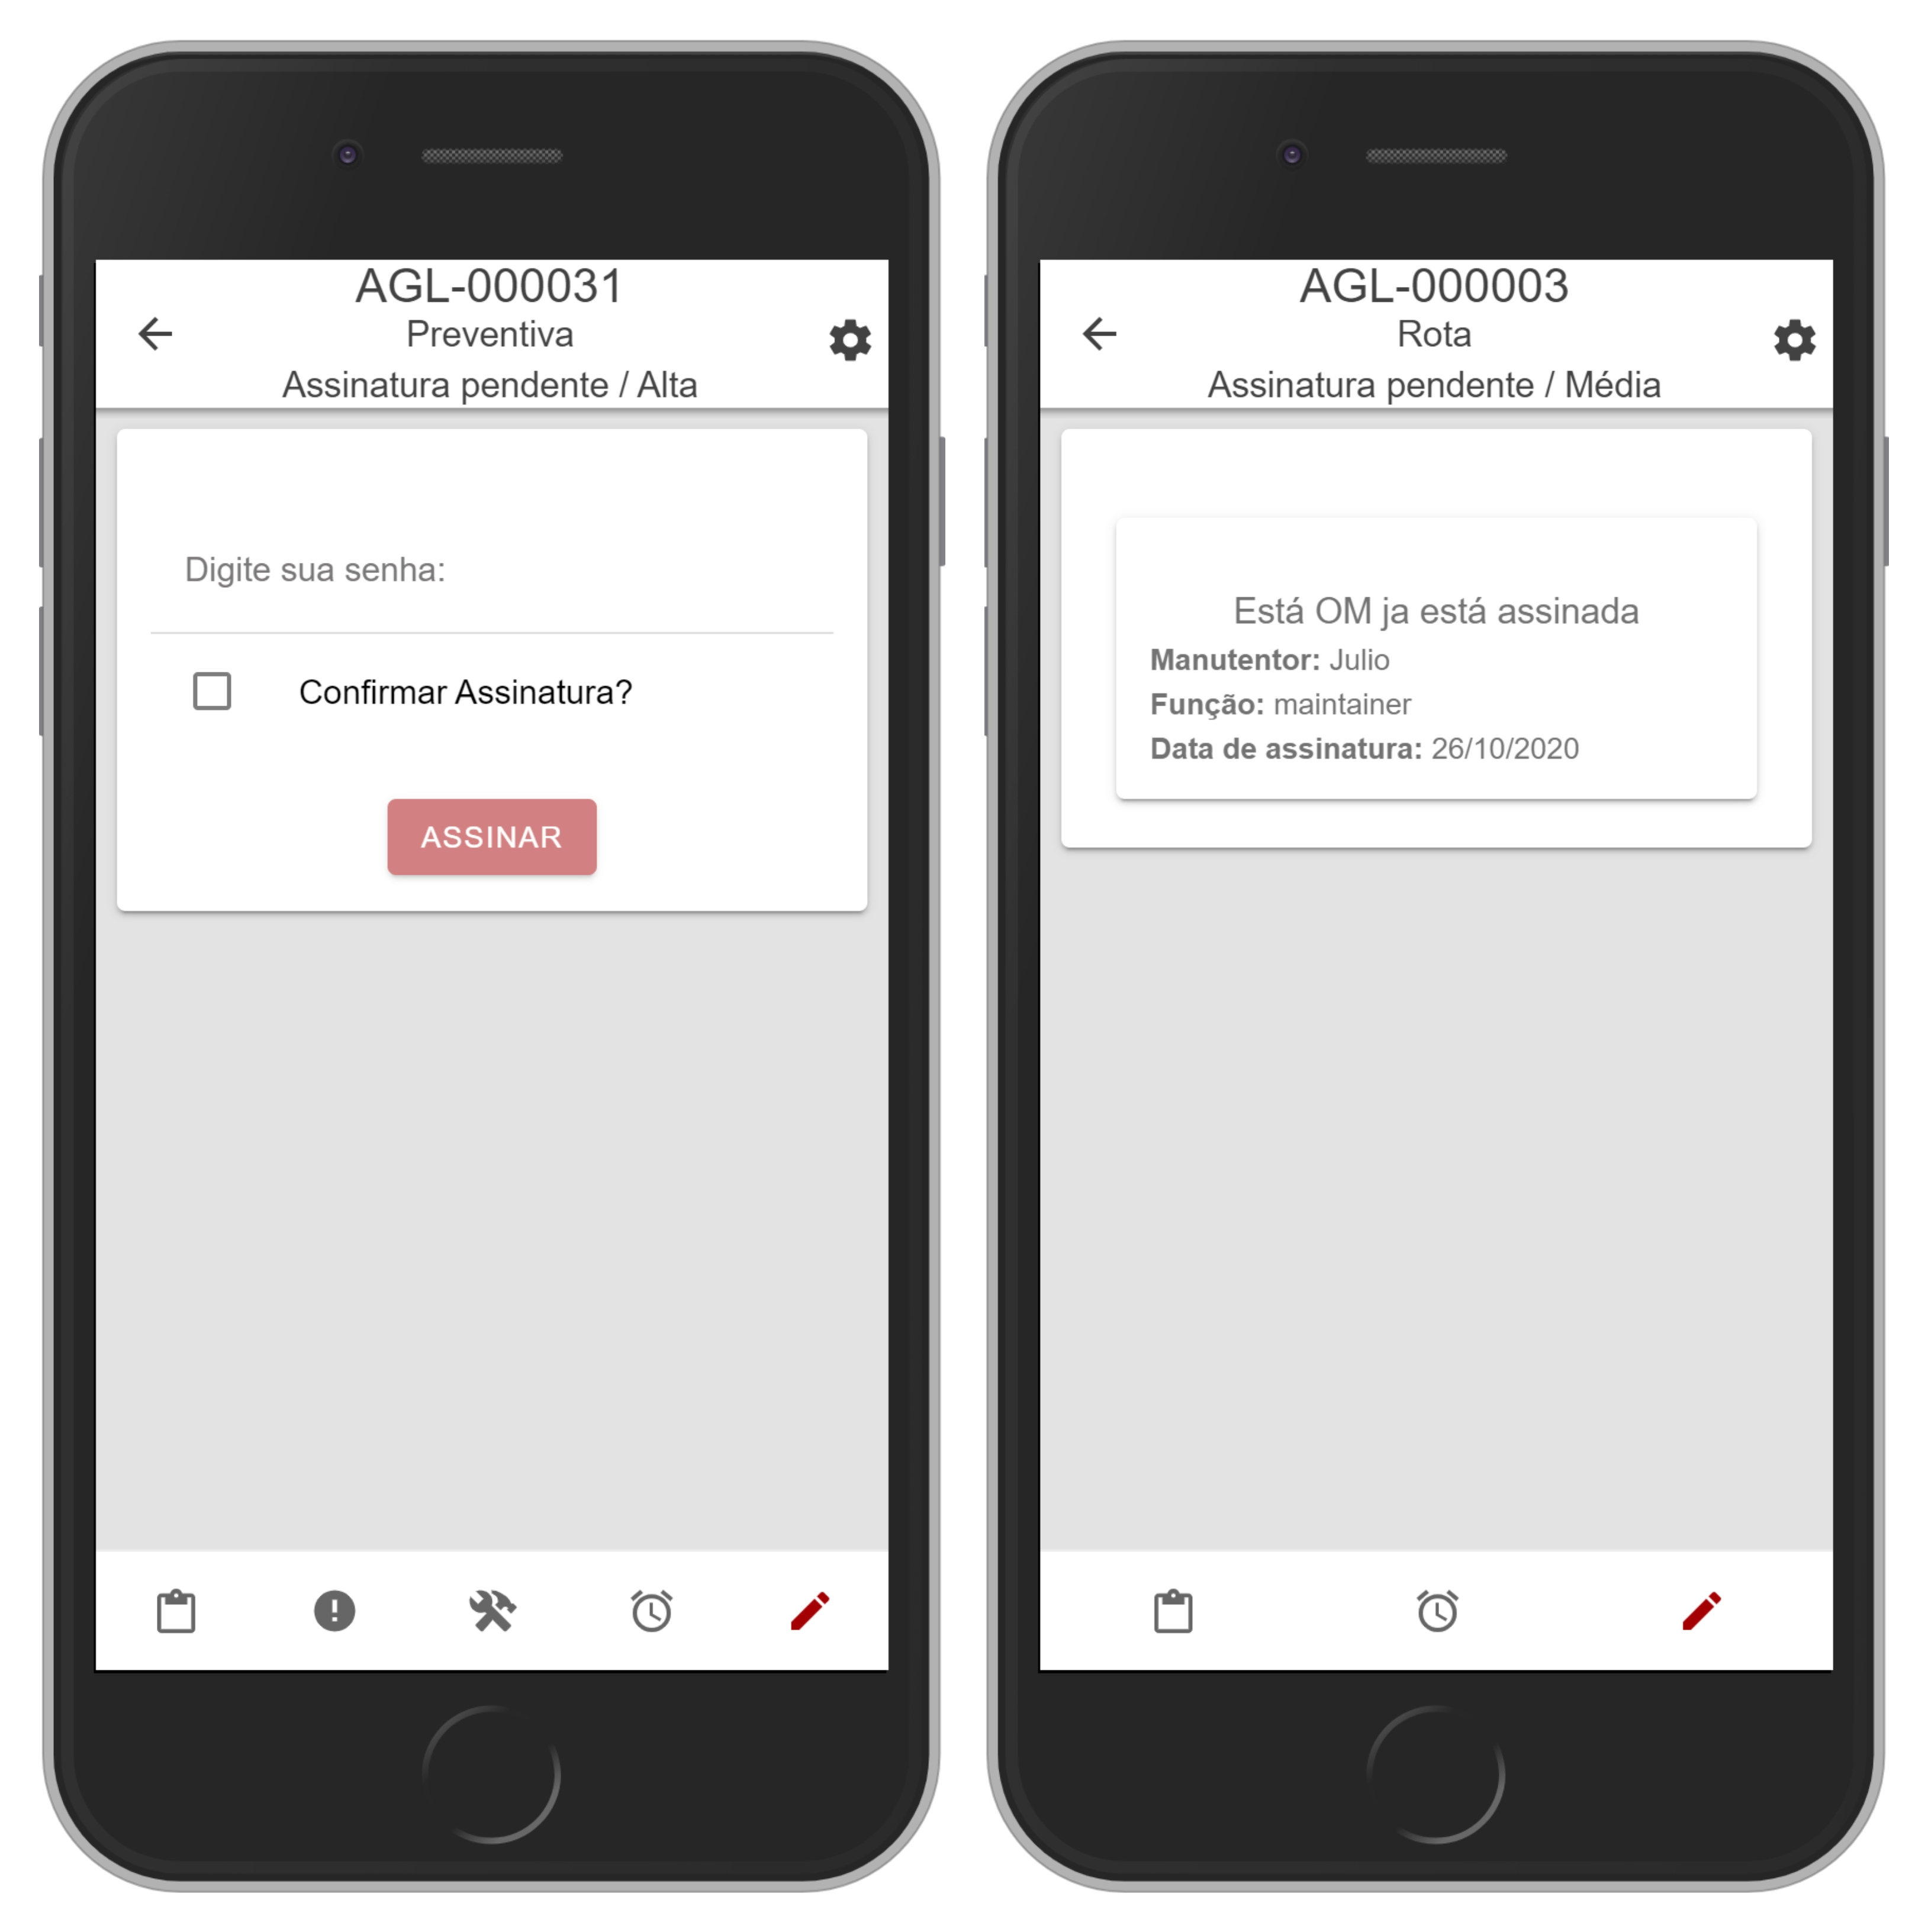
\includegraphics[scale=0.55]{./Figuras/agil.it/mobile-om-assinatura.jpg}
	\end{center}
	\legend{Fonte: os autores (2020)}
\end{figure}

A figura \ref{mobile-om-assinatura} mostra o processo de assinatura da ordem, caso ainda não tenha sido assinada será apresentado para assinatura, no qual o técnico deve informar a senha dele e marcar a caixa para confirmar a assinatura e clicar no botão ``Assinar''. Caso já esteja assinada, será informada as assinaturas da ordem contendo os dados do usuário que assinou e sua função e a data da assinatura.